% !TeX root = ../../Book2.tex
% 纲要标题：## 附录 C　等变拓扑、稳定结构与计算
% 纲要位置：几何学计划纲要.md，第 2036 行。
% 正文状态：初稿；正文、证明、例子及习题解答已写，尚未正式审核。
% 补充范围与先修：等变 de Rham 与 Cartan 模型固定紧 Lie 群的光滑作用及实系数；与 Borel 构造的比较明确所用有限维逼近和不变性条件。环面局部化另列紧性、定向、固定点分支及系数局部化条件；具体积分公式的主要证明和辛几何应用放第四卷矩映射与局部化，不与稳定同伦、持续同调支线混用。

% 纲要内容开始
% 
% > 保持三条支线独立，不用一个共同定义掩盖三种不同的稳定化。
% 
% > 补充写作范围与外部输入：等变 de Rham 与 Cartan 模型固定紧 Lie 群光滑作用及实系数，说明与 Borel 构造比较的条件；环面局部化另列系数、紧性、定向和固定点分支条件。积分公式的主要证明及辛几何应用放第四卷矩映射与局部化，不与稳定同伦、持续同调支线混用。
% 
% * **等变上同调**
%   * Borel 构造及纤维序列
%   * 固定点和自由作用的对照
%   * 圆群等变球面算例
%   * 等变 de Rham 复形与 Cartan 模型
%   * 紧 Lie 群作用下的比较条件
%   * 环面局部化所需的系数与紧性条件
% 
% * **谱与稳定同伦**
%   * 悬挂稳定化和谱
%   * 稳定同伦群及系数谱
%   * 广义同调理论的进一步输入
% 
% * **持续同调的代数结构**
%   * 有限滤过复形及诱导映射
%   * 域系数条形码的分解
%   * 边界矩阵约化
%   * 稳定性需要的距离与有限性条件
% 
% ---
% 
% 纲要内容结束

\chapter{等变拓扑、稳定结构与计算}
\label{g2:app:C}
\BookChapterNumber{g2:app:C}

\begin{chapterabstract}
	群作用、悬挂与滤过给拓扑不变量提出了三类进一步的问题。等变上同调通过 Borel 构造保存稳定子信息，圆群作用的球面计算将它化为射影丛关系；Cartan 模型以微分形式实现同一理论，局部化说明固定点数据何时足以恢复整体。谱将反复悬挂后的同伦数据组织起来，球谱、普通同调谱与周期 K 理论谱展示不同的系数行为。持续同调则保存滤过中同调类的出现与消失，以区间分解和边界矩阵约化得到条形码，并用交错与瓶颈距离表达扰动稳定性。
\end{chapterabstract}

\begin{learninggoals}
	\begin{itemize}
		\item 从关联丛构造 \(X_G\)，比较自由轨道与固定点，计算圆群等变球面的环及固定点限制。
		\item 写出 Cartan 复形的分次、群不变性与微分，核验平方为零，说明紧群比较及环面局部化的适用条件。
		\item 从悬挂过渡映射定义谱的稳定同伦群，用球谱、普通同调谱和 K 理论谱辨认系数及次数。
		\item 将有限滤过转为向量空间及线性映射，分解为区间模，并从秩函数读出区间重数。
		\item 手工约化边界矩阵，解释出生与死亡配对，使用交错和瓶颈距离估计过滤值扰动的影响。
	\end{itemize}
\end{learninggoals}

当圆群旋转一个球面时，纬圈都成为轨道，南北两极却保持不动。若只计算轨道空间的上同调，这种区别几乎全部消失。另一方面，将一个带基点空间反复悬挂，有些原本依赖维数的同伦群会进入稳定范围。再看一个逐次加入顶点、边和面的复形：最终同调能够说明剩下几个洞，却不能告诉我们这些洞何时出现、何时被填掉。本附录分别为这三个问题建立合适的对象。

\ProseParagraphBreak

三节可以按需要分别阅读。等变部分使用第7章 de Rham 理论、第19章主丛分类、第20—21章 Thom 类与射影丛公式；稳定同伦部分使用第8—12章的悬挂、同伦群与表示空间，K 理论例子另接第24章；持续同调部分主要使用第2章链复形及有限维线性代数。每一条支线的“稳定”都有自己的含义，下面的对应关系有助于在阅读中保持对象和任务的一致。

\begin{table}[htbp]
	\centering
	\caption{三条支线的对象与比较方式}
	\label{g2:tab:appendix-c-three-directions}
	\begin{tabularx}{\textwidth}{@{}lXX@{}}
		\toprule
		支线 & 加入的数据 & 所研究的比较 \\
		\midrule
		等变上同调 & 群作用、稳定子与通用主丛 & 与普通商、固定点及微分形式模型的比较 \\
		谱与稳定同伦 & 空间序列及悬挂结构映射 & 反复悬挂后的同伦类及广义同调 \\
		持续同调 & 同一滤过中各次包含诱导的映射 & 区间分解以及过滤值扰动后的条形码距离 \\
		\bottomrule
	\end{tabularx}
\end{table}

本附录完整展开代表模型和有限代数计算。紧群的等变 de Rham 比较、紧光滑环面作用的局部化、稳定同伦范畴的基础构造以及条形码匹配定理，在实际使用处列明所选版本和证明输入。等变积分的主要证明及辛约化应用接第四卷第12.6节；持续同调与 Floer 作用滤过的联系接第四卷附录 E。

\section{等变上同调}
\label{g2:sec:C01}

一点上的平凡圆群作用与圆周上的自由旋转，轨道空间都是一点。前者的点被整个圆群固定，后者的点只有单位元保持不动，这个差别在取商时消失了。等变上同调用一个同时保存空间与群作用的构造代替普通商空间。圆群作用于二球面的例子会把这种信息写成一条明确的环关系。

\subsection{Borel 构造及纤维序列}
\label{g2:subsec:C01:01}

取紧矩阵 Lie 群 \(G\)，并取第19章构造的通用主右丛 \(EG\to BG\)。\cref{g2:prop:universal-matrix-principal-bundle}已经证明：\(EG\) 可缩，右 \(G\) 作用自由，而且轨道映射局部平凡。可缩性使这一辅助空间不增加普通同伦信息；自由性则让对角作用能够取一个保留群数据的商。

\begin{definition}\label{g2:def:borel-construction}
	设 \(X\) 是左 \(G\) 空间。其\term[Borel gouzao]{Borel 构造}[Borel construction]，也称同伦商，定义为
	\[
		X_G=EG\times_GX=(EG\times X)/\!\sim,
		\qquad(eg,x)\sim(e,gx).
	\]
	等价地，商掉的是自由右作用 \((e,x)g=(eg,g^{-1}x)\)。对含幺交换环 \(R\)，定义\term[dengbianshangtongdiao]{等变上同调}[equivariant cohomology]
	\[
		H_G^*(X;R)=H^*(X_G;R).
	\]
	右端是普通奇异上同调，乘法为杯积。\symidx{\(X_G=EG\times_GX\)：Borel 构造}\symidx{\(H_G^*(X;R)\)：等变上同调}
\end{definition}

这个构造沿用第19章的关联丛关系，左右作用的次序因而已有固定含义。名称中的 Borel 指 Armand Borel。\footnote{Armand Borel（1923--2003），瑞士数学家，研究代数拓扑与线性代数群。}投影
\[
	p:X_G\longrightarrow BG,\qquad[e,x]\longmapsto[e]
\]
把 \(X_G\) 组织成纤维为 \(X\) 的关联丛：若 \(s:V\to EG\) 是局部截面，便有丛图
\[
	V\times X\longrightarrow p^{-1}(V),\qquad(b,x)\longmapsto[s(b),x].
\]
若 \(e=s(b)g\)，其逆把 \([e,x]\) 送到 \((b,gx)\)。这也直接核验了丛图与商关系相容。

\ProseParagraphBreak

由\cref{g2:thm:bundle-serre}，上述纤维丛是 Serre 纤维化。选定 \(e_0\in EG\) 后，\(x\mapsto[e_0,x]\) 把 \(X\) 识别为 \([e_0]\) 上的纤维，故有纤维序列
\begin{equation}\label{g2:eq:borel-fiber-sequence}
	X\longrightarrow X_G\xrightarrow{p}BG.
\end{equation}
这里“纤维序列”说明 \(X\) 也代表 \(p\) 的同伦纤维；它给出第8章的同伦长正合列，并可使用第11章的纤维化谱序列。它并没有把 \(X_G\) 写成 \(X\times BG\)，作用的粘合数据仍在过渡函数里。

\begin{proposition}\label{g2:prop:borel-model-independence}
	若 \(EG\) 与 \(E'G\) 都是可缩、自由且轨道映射局部平凡的通用主 \(G\) 空间，则它们所给的 \(H_G^*(X;R)\) 自然同构。连续等变映射 \(a:X\to Y\) 诱导上同调环同态 \(a_G^*:H_G^*(Y;R)\to H_G^*(X;R)\)，等变同伦的映射诱导相同同态。
\end{proposition}
\begin{proof}
	比较空间取 \((EG\times E'G\times X)/G\)，其中右作用为
	\[
		(e,e',x)g=(eg,e'g,g^{-1}x).
	\]
	忘记 \(e'\) 或 \(e\) 分别得到映到两种 Borel 构造的纤维丛，纤维分别为 \(E'G\) 与 \(EG\)。例如在第一种 Borel 构造上，这张丛来自将主丛 \(EG\to BG\) 沿 \(p\) 拉回后，以 \(E'G\) 为关联纤维；局部丛图给出所需平凡化。两个纤维都可缩，纤维化同伦长正合列说明两个投影在全部同伦群与道路分支上诱导同构。依\cref{g2:lem:weak-equivalence-homology}，弱同伦等价诱导奇异同调同构，再由上同调万有系数定理得到任意 \(R\) 系数上同调同构；这些同构保持杯积。

	等变映射给出 \([e,x]\mapsto[e,a(x)]\)，等变同伦则以同一公式下降为 Borel 构造间的同伦。投影比较与这些映射交换，因而同构自然；对三个辅助空间用三重乘积比较，又保证不同次比较彼此相容。
\end{proof}

投影的拉回 \(p^*:H^*(BG;R)\to H_G^*(X;R)\) 使等变上同调成为 \(H^*(BG;R)\) 上的代数。纤维包含则给出
\[
	j^*:H_G^*(X;R)\longrightarrow H^*(X;R),
\]
称为忘却映射。它把辅助的群参数忘掉。因 \(p\circ j\) 是常映射，来自 \(H^{>0}(BG;R)\) 的类都映为零；但是忘却映射未必满射，因此一般不能只把群参数置零就得到全部普通上同调。

\subsection{固定点和自由作用的对照}
\label{g2:subsec:C01:02}

若作用平凡，商关系只作用于 \(EG\) 这一因子，故直接得到
\[
	X_G=BG\times X.
\]
例如 \(H_G^*(\mathrm{pt};R)=H^*(BG;R)\)。对域 \(k\) 和有限 CW 复形 \(X\)，Künneth 公式还给出
\[
	H_G^*(X;k)=H^*(BG;k)\otimes_kH^*(X;k)
\]
作为分次代数的同构；乘法含通常的分次交换符号。有限性保证每个总次数只需处理有限维纤维同调，普通上同调的张量表达因而适用。

\begin{proposition}\label{g2:prop:free-action-borel-quotient}
	设紧 Lie 群 \(G\) 在 \(X\) 上自由左作用，且 \(X\to X/G\) 是局部平凡主丛。则
	\[
		q:X_G\longrightarrow X/G,\qquad[e,x]\longmapsto Gx
	\]
	是纤维为 \(EG\) 的局部平凡纤维丛，因而诱导自然环同构
	\[
		q^*:H^*(X/G;R)\xrightarrow{\ \cong\ }H_G^*(X;R).
	\]
\end{proposition}
\begin{proof}
	在 \(X/G\) 的开集 \(V\) 上取截面 \(s\)。每个 \(x\) 唯一写成 \(g s(b)\)，其中 \(b=Gx\)。于是
	\[
		q^{-1}(V)\longrightarrow V\times EG,\qquad
		[e,g s(b)]\longmapsto(b,eg)
	\]
	良定义，逆为 \((b,e)\mapsto[e,s(b)]\)。因此 \(q\) 是所述纤维丛。\(EG\) 可缩，故由同伦长正合列及弱等价的同调判据，\(q\) 在上同调上诱导同构；自然性和环结构均来自连续映射的拉回。
\end{proof}

对于圆群 \(T=S^1\)，可取 \(ET=S^\infty\)、\(BT=\mathbb CP^\infty\)，右作用是单位复数的标量乘法。若 \(T\) 在一点上平凡作用，等变上同调是 \(H^*(BT;\mathbb Z)\cong\mathbb Z[u]\)，其中 \(|u|=2\)。若 \(T\) 在自身上以左乘作用，映射 \([e,z]\mapsto ez\) 把 \(T_T\) 同胚到 \(ET\)，所以其等变上同调只有零次的 \(\mathbb Z\)。这两个作用的轨道空间都是一点，等变上同调却清楚地区分了它们。后一例的忘却映射不能得到 \(H^1(S^1;\mathbb Z)\) 的生成元。

\ProseParagraphBreak

固定点则产生相反的现象。若 \(x\in X\) 被整个 \(G\) 固定，映射
\[
	s_x:BG\longrightarrow X_G,\qquad[e]\longmapsto[e,x]
\]
满足 \(p\circ s_x=\operatorname{id}\)，所以 \(p^*\) 单射。更一般地，令 \(X^G=\{x:gx=x\text{ 对所有 }g\in G\}\)，其包含诱导
\[
	H_G^*(X;R)\longrightarrow H_G^*(X^G;R)
	=H^*(BG\times X^G;R).
\]
固定点上的这些限制可以用于检测整体等变类。

\begin{proposition}\label{g2:prop:borel-homogeneous-orbit}
	设 \(H\subset G\) 为闭子群，\(G\) 在 \(G/H\) 上左乘。则
	\[
		(G/H)_G\cong EG/H,
		\qquad H_G^*(G/H;R)\cong H^*(BH;R).
	\]
	在这个识别下，\(H^*(BG;R)\) 的作用来自自然投影 \(EG/H\to EG/G\) 的拉回。
\end{proposition}
\begin{proof}
	定义 \([e,gH]\mapsto egH\)。关系 \([ea,gH]=[e,agH]\) 的两边都映到 \(eagH\)，故映射良定义；其逆为 \(eH\mapsto[e,H]\)，两者在商拓扑中连续且互逆。\(EG\) 作为 \(H\) 空间仍自由、可缩，\(EG\to EG/H\) 由闭子群商的局部截面给出主 \(H\) 丛，因此可以作 \(EH\to BH\) 的模型。最后的代数结构由同一个投影公式得到。
\end{proof}

这个公式把每条轨道上留下的信息解释为稳定子 \(H\) 的分类空间。当 \(H=G\) 时得到一个固定点的 \(BG\)，当 \(H=\{1\}\) 时得到自由轨道的可缩空间。介于二者之间的稳定子也会留下相应信息。用普通轨道空间替换 Borel 构造，会把这些不同的分类空间全部压成一点。

\subsection{圆群等变球面算例}
\label{g2:subsec:C01:03}

取 \(T=S^1\) 在 \(S^2=\mathbb CP^1\) 上的作用
\[
	z\cdot[z_0:z_1]=[z_0:zz_1].
\]
它的固定点为 \(N=[1:0]\)、\(S=[0:1]\)，其余轨道都是纬圈，轨道空间为闭区间。为了计算等变上同调，先把这张球面上的作用转为 \(BT\) 上的一张射影丛。

\ProseParagraphBreak

记 \(\mathbb C_1\) 为权 \(1\) 的表示，即 \(z\) 作用为乘以 \(z\)，并固定
\begin{equation}\label{g2:eq:equivariant-circle-generator}
	L=ET\times_T\mathbb C_1,\qquad u=c_1(L)\in H^2(BT;\mathbb Z).
\end{equation}
\symidx{\(u=c_1(ET\times_T\mathbb C_1)\)：圆群的二次系数生成元}
在 \(ET=S^\infty\) 的右标量模型中，\([e,w]\mapsto we\) 将 \(L\) 识别为 \(\mathbb CP^\infty\) 的重言线丛 \(\gamma\)。因此若第21章的正生成元记作 \(h=c_1(\gamma^*)\)，本节的 \(u=-h\)。给出这项符号选择，是为了同时读出表示权、固定点限制与后面的 Cartan 变量。

\begin{theorem}\label{g2:thm:equivariant-sphere-ring}
	对上述圆群作用及式\eqref{g2:eq:equivariant-circle-generator}的生成元，存在二次类 \(x\)，使
	\begin{equation}\label{g2:eq:equivariant-sphere-ring}
		H_T^*(S^2;\mathbb Z)\cong\mathbb Z[u,x]/\bigl(x(x+u)\bigr),
		\qquad |u|=|x|=2.
	\end{equation}
	作为 \(\mathbb Z[u]\) 模，它以 \(1,x\) 为基。忘却映射将 \(u\) 送到零、将 \(x\) 送到 \(H^2(\mathbb CP^1;\mathbb Z)\) 的复定向正生成元。固定点限制为
	\begin{equation}\label{g2:eq:sphere-fixed-restriction}
		i^*(a(u)+x b(u))=\bigl(a(u),a(u)-u b(u)\bigr).
	\end{equation}
\end{theorem}
\begin{proof}
	球面是表示 \(\mathbb C_0\oplus\mathbb C_1\) 的线子空间射影空间。取关联丛与取线子空间相容，故
	\[
		(S^2)_T\cong\mathbb P(\underline{\mathbb C}\oplus L).
	\]
	具体地，\([e,\ell]\) 对应于关联纤维中由 \([e,v]\)、\(v\in\ell\) 组成的线。更换代表 \(e\) 时，\(\ell\) 同时按群作用变化，所以这条线保持不变；局部平凡化给出连续的逆。

	令 \(\lambda\) 为这张射影丛上的重言线丛，取 \(x=c_1(\lambda^*)\)。\cref{g2:thm:projective-bundle}给出模基 \(1,x\)，\cref{g2:def:chern-classes-projective}则将射影丛关系的系数识别为 \(E=\underline{\mathbb C}\oplus L\) 的陈类。由直和公式，\(c_1(E)=u\)、\(c_2(E)=0\)，于是
	\[
		x^2+ux=0.
	\]
	\(H^*(BT;\mathbb Z)=\mathbb Z[u]\) 来自\cref{g2:thm:complex-projective-ring}在无限射影空间上的计算，所以得到所述环。纤维上的 \(\lambda\) 是通常的重言线丛，因此 \(x\) 限制为正生成元。

	固定点 \(N\) 对应于 \(E\) 的平凡线，\(S\) 对应于 \(L\)。在这两个截面上，\(\lambda^*\) 分别限制为平凡线和 \(L^*\)，故
	\[
		x|_N=0,\qquad x|_S=-u.
	\]
	\(u\) 从底空间拉回，在两个截面上仍为 \(u\)。代入模基的唯一表达即得式\eqref{g2:eq:sphere-fixed-restriction}。
\end{proof}

限制到固定点究竟丢失多少信息，现在可以逐项计算。若 \(i^*(a+xb)=0\)，第一分量给 \(a=0\)，第二分量给 \(ub=0\)。\(\mathbb Z[u]\) 没有零因子，故 \(b=0\)，所以此例的固定点限制单射。它的像是
\begin{equation}\label{g2:eq:sphere-congruence-image}
	\{(P,Q)\in\mathbb Z[u]\oplus\mathbb Z[u]:P-Q\text{ 能被 }u\text{ 整除}\}.
\end{equation}
若差能被 \(u\) 整除，取 \(a=P\)、\(b=(P-Q)/u\) 就得到原像，证明这一描述也充分。两个固定点的类因而还要满足一条粘合关系。

\ProseParagraphBreak

将 \(u\) 变为可逆元后，每一对 Laurent 多项式都满足上述可解性条件，故
\[
	H_T^*(S^2;\mathbb Z)[u^{-1}]
	\cong\mathbb Z[u,u^{-1}]\oplus\mathbb Z[u,u^{-1}].
\]
右侧两份系数环由两个固定点分别贡献。对应于 \((1,0)\)、\((0,1)\) 的类是
\[
	e_N=\frac{x+u}{u},\qquad e_S=-\frac{x}{u}.
\]
利用 \(x(x+u)=0\) 可直接验证 \(e_N+e_S=1\)、\(e_Ne_S=0\)、\(e_N^2=e_N\)、\(e_S^2=e_S\)。这是局部化之后整体环分成固定点两部分的一个完整计算。

\begin{figure}[htbp]
	\centering
	% !TeX root = ../Book2.tex
\begin{tikzpicture}[>=stealth,every node/.style={font=\small}]
	\shade[ball color=blue!10] (0,0) circle (1.45);
	\draw[thick] (0,0) circle (1.45);
	\draw[dashed,gray] (-1.45,0) arc (180:0:1.45 and .4);
	\draw[blue!70!black,->] (1.45,0) arc (0:-165:1.45 and .4);
	\fill (0,1.45) circle (2pt) node[above] {\(N\)};
	\fill (0,-1.45) circle (2pt) node[below] {\(S\)};
	\draw[->] (1.85,0)--(3.15,0) node[midway,above] {取轨道};
	\draw[very thick] (3.65,-1.45)--(3.65,1.45);
	\fill (3.65,1.45) circle (2pt) node[above] {\(N\)};
	\fill (3.65,-1.45) circle (2pt) node[below] {\(S\)};
	\node[right] at (4.35,.65) {\(x|_N=0\)};
	\node[right] at (4.35,-.65) {\(x|_S=-u\)};
	\node at (2.8,-2.1) {\(i^*(a+xb)=(a,a-ub)\)};
\end{tikzpicture}

	\caption{圆群沿纬圈旋转二球面。普通商把每条纬圈压为区间中的一点；固定点限制则给出两份 \(\mathbb Z[u]\)，在局部化之前还须满足 \(P-Q\in u\mathbb Z[u]\) 的关系。}
	\label{g2:fig:equivariant-sphere}
\end{figure}

若圆群在同一个球面上平凡作用，得到的却是 \(\mathbb Z[u,x]/(x^2)\)。两种作用的普通空间相同，区别写在 \(ux\) 这一项里；取商得到的区间又没有这种二次信息。在后面的微分形式模型中，关系中的 \(u\) 将成为记录无穷小群作用的多项式变量，而 \(x\) 会有一个可显式写出的等变闭代表。

\subsection{等变 de Rham 复形与 Cartan 模型}
\label{g2:subsec:C01:04}

Borel 构造给出了等变上同调的拓扑定义。若群与流形都是光滑的，还可以寻找一种由微分形式组成的计算模型。不过，单取不变微分形式并不够：一点上的微分形式只有常数，而 \(H_{S^1}^*(\mathrm{pt};\mathbb R)=\mathbb R[u]\) 在每个非负偶数次都有类。模型必须同时容纳流形上的形式与群方向的多项式。

\ProseParagraphBreak
设 \(G\) 是 Lie 群，\(\mathfrak g\) 是其 Lie 代数，\(M\) 是有限维 Hausdorff、第二可数光滑无边流形，并给定光滑左作用 \(a_g\colon M\to M\)。本节固定基本向量场的符号
\begin{equation}\label{g2:eq:cartan-fundamental-field}
	\xi_M(x)=\left.\frac{\mathrm d}{\mathrm dt}\right|_{t=0}\exp(t\xi)\cdot x,
	\qquad \xi\in\mathfrak g.
\end{equation}
把 \(S(\mathfrak g^*)\otimes\Omega(M)\) 中的元素看成以 \(\xi\in\mathfrak g\) 为变量、取值于微分形式的多项式 \(\alpha(\xi)\)。其中一个线性多项式的次数规定为 \(2\)，一个普通 \(b\) 次形式的次数仍为 \(b\)。这样规定的原因将在微分中显现：插入 \(\xi_M\) 降低一个形式次数，同时增加一个多项式次数，合计提高一次。

\begin{definition}\label{g2:def:cartan-complex}
	\term[Cartan moxing]{Cartan 模型}[Cartan model]的次数 \(k\) 部分为
	\[
		\Omega_G^k(M)=\bigoplus_{2a+b=k}\bigl(S^a(\mathfrak g^*)\otimes\Omega^b(M)\bigr)^G.
	\]
	这里上标 \(G\) 要求多项式满足
	\begin{equation}\label{g2:eq:cartan-equivariant-polynomial}
		a_g^*\alpha(\operatorname{Ad}_g\xi)=\alpha(\xi)
		\qquad(g\in G,\ \xi\in\mathfrak g).
	\end{equation}
	在这个空间上定义\term[dengbian weifen]{等变微分}[equivariant differential]
	\begin{equation}\label{g2:eq:cartan-differential}
		(\mathrm d_G\alpha)(\xi)=\mathrm d\bigl(\alpha(\xi)\bigr)-\iota_{\xi_M}\alpha(\xi).
	\end{equation}
\end{definition}

这里的 Cartan 指 Henri Cartan。\footnote{Henri Cartan（1904--2008），法国数学家，在多复变函数、层论和代数拓扑中有重要贡献。等变上同调的 Cartan 模型来自他的工作。}第一卷使用的 Cartan 公式则属于微分形式的运算规则。为便于在这里使用，回忆第一卷第14.1节已经证明
\[
	\mathcal L_X=\mathrm d\iota_X+\iota_X\mathrm d,
\]
其中 \(\mathcal L_X\) 由向量场正向流的拉回求导定义。这个符号与式\eqref{g2:eq:cartan-fundamental-field}一致。

\begin{proposition}\label{g2:prop:cartan-is-complex}
	\(\mathrm d_G\) 保持式\eqref{g2:eq:cartan-equivariant-polynomial}的条件，是次数 \(1\) 的分次导子，并且在 \(\Omega_G(M)\) 上满足 \(\mathrm d_G^2=0\)。因而 \((\Omega_G(M),\mathrm d_G)\) 是分次交换微分代数。
\end{proposition}
\begin{proof}
	基本向量场满足 \((a_g)_*\xi_M=(\operatorname{Ad}_g\xi)_M\)，所以外微分和插入运算都与式\eqref{g2:eq:cartan-equivariant-polynomial}相容。若选择 \(\mathfrak g\) 的基 \(e_1,\ldots,e_r\)，相应线性坐标为 \(u_1,\ldots,u_r\)，则
	\[
		\mathrm d_G=\mathrm d-\sum_{j=1}^r u_j\iota_{(e_j)_M}.
	\]
	每一项的总次数都是 \(1\)。外微分与插入都是按形式次数取符号的导子，而多项式次数为偶数，故该符号也就是按总次数取的符号。

	固定 \(\xi\) 后，\(\mathrm d^2=0\)、\(\iota_{\xi_M}^2=0\) 与 Cartan 公式给出
	\[
		(\mathrm d_G^2\alpha)(\xi)=-\mathcal L_{\xi_M}\alpha(\xi).
	\]
	在等变性条件中取 \(g=\exp(t\xi)\)。由于 \(\operatorname{Ad}_{\exp(t\xi)}\xi=\xi\)，得到 \(a_{\exp(t\xi)}^*\alpha(\xi)=\alpha(\xi)\)。对 \(t\) 求导便得右端为零。
\end{proof}

这也解释了为何定义要取 \(G\) 不变部分：在任意多项式值形式上，\(\mathrm d_G^2\) 通常只是 \(-\mathcal L_{\xi_M}\)，并不为零。还应区分不变性与水平性。一个普通形式 \(\beta\) 称为\term[jiben xingshi]{基本形式}[basic form]，是指它既满足 \(a_g^*\beta=\beta\)，又满足所有 \(\iota_{\xi_M}\beta=0\)。自由适当作用下，基本形式恰是商流形上的形式的拉回。Cartan 模型要求的是式\eqref{g2:eq:cartan-equivariant-polynomial}，并未逐项要求水平；插入项正用来记录沿轨道方向的变化。

\begin{example}\label{g2:ex:cartan-point-circle}
	在一点上，\(\Omega_G(\mathrm{pt})=S(\mathfrak g^*)^G\)，微分为零。特别地，令 \(T=S^1=\mathbb R/\mathbb Z\)，取满足 \(\exp(t\xi)=e^{2\pi it}\) 的生成元，并以 \(u(\xi)=1\) 规定线性坐标，则模型为 \(\mathbb R[u]\)，\(\lvert u\rvert=2\)。这里的 \(u\) 将在下一小节与前文权 \(1\) 关联线的一阶陈类相认。

	若 \(T\) 左平移作用于自身，令 \(\theta\in\mathbb R/\mathbb Z\) 为角坐标。虽然 \(\theta\) 不是全局实值函数，\(\mathrm d\theta\) 却是全局形式；不变形式由 \(1\) 与 \(\mathrm d\theta\) 张成，且
	\[
		\mathrm d_T(\mathrm d\theta)=-u.
	\]
	复形为 \(\mathbb R[u]\otimes\Lambda(\mathrm d\theta)\)：所有正次 \(u^j\) 都是边界，奇次没有非零闭元，所以其上同调只有零次的 \(\mathbb R\)。这与自由作用的商是一点相符。
\end{example}

\begin{example}\label{g2:ex:cartan-rotating-sphere}
	继续取式\eqref{g2:eq:sphere-fixed-restriction}中的圆群作用
	\[
		z\cdot[z_0:z_1]=[z_0:zz_1].
	\]
	在两极之外设
	\[
		s=\frac{|z_1|^2}{|z_0|^2+|z_1|^2},\qquad
		\theta=\frac{\arg(z_1/z_0)}{2\pi},\qquad
		\omega=\mathrm ds\wedge\mathrm d\theta.
	\]
	\(s\) 从北极 \(N=[1:0]\) 的 \(0\) 增至南极 \(S=[0:1]\) 的 \(1\)。虽然角坐标在两极失效，\(\omega\) 却光滑延拓到整个球面：在 \(w=z_1/z_0=x+iy\) 坐标中，
	\[
		\omega=\frac{1}{\pi(1+|w|^2)^2}\,\mathrm dx\wedge\mathrm dy,
	\]
	改用 \(1/w\) 后仍是同型表达式。它按复定向满足 \(\int_{\mathbb CP^1}\omega=1\)。基本向量场为 \(V=\partial_\theta\)，因而
	\[
		\iota_V\omega=-\mathrm ds=\mathrm d\mu,\qquad \mu=-s.
	\]
	于是总次数为 \(2\) 的多项式值形式
	\begin{equation}\label{g2:eq:cartan-sphere-form}
		\widetilde\omega=\omega+u\mu=\omega-su
	\end{equation}
	满足 \(\mathrm d_T\widetilde\omega=u(\mathrm d\mu-\iota_V\omega)=0\)。其固定点限制是 \(0\) 与 \(-u\)。这里零次形式 \(\mu\) 恰好抵消了 \(\omega\) 沿轨道方向的插入；这就是等变闭形式比普通闭形式多出一个多项式项的具体原因。
\end{example}

\subsection{紧 Lie 群作用下的比较条件}
\label{g2:subsec:C01:05}

Cartan 复形可以按定义对任意 Lie 群写下。它何时计算 Borel 上同调，则需要比较定理。以下等变 de Rham 定理的紧连通版本取自 Meinrenken\cite[\S6, Theorem 6.1]{Meinrenken2006EquivariantCartan}；Atiyah--Bott\cite[\S4, Theorem 4.13]{AtiyahBott1984MomentMap}给出了等价的 Weil 模型版本。两者的基本场符号须与式\eqref{g2:eq:cartan-fundamental-field}配套，下面用圆群连接把本书的归一化具体写出。

\begin{theorem}[等变 de Rham 定理]\label{g2:thm:equivariant-de-rham}
	设紧 Lie 群 \(G\) 光滑作用于有限维 Hausdorff、第二可数光滑无边流形 \(M\)。则有自然的分次环同构
	\[
		H^*(\Omega_G(M),\mathrm d_G)\cong H_G^*(M;\mathbb R).
	\]
	该同构与等变光滑映射的拉回相容，也与来自一点的系数环作用相容。这里不要求 \(M\) 紧、作用自由或 \(M\) 定向。
\end{theorem}

引用文献的紧连通版本可以推出这里的全部紧群版本。事实上，令 \(G^\circ\) 为单位连通分支，\(\Gamma=G/G^\circ\) 为有限群。Lie 代数相同，并且
\[
	\Omega_G(M)=\Omega_{G^\circ}(M)^\Gamma.
\]
对有限群取不变量在实向量空间上是正合的：用 \(|\Gamma|^{-1}\sum_{\gamma\in\Gamma}\gamma\) 平均即可把不变的上同调类选成不变代表，并把不变边界选成不变原像。因此左端的上同调是 \(H^*(\Omega_{G^\circ}(M))^\Gamma\)。拓扑一侧有正则有限覆盖
\[
	EG\times_{G^\circ}M\longrightarrow EG\times_G M
\]
及覆盖变换群 \(\Gamma\)。有限覆盖的转移满足“拉回后求和”与“先转移再拉回”的关系，除以 \(|\Gamma|\) 后给出
\[
	H_G^*(M;\mathbb R)\cong H_{G^\circ}^*(M;\mathbb R)^\Gamma.
\]
连通版本的比较同构具有自然性，因而与这两个 \(\Gamma\) 作用相容，遂得所述结论。对非连通群只保留 Lie 代数的不变性会漏掉这个有限群作用；定义中取整个 \(G\) 的不变量正为此所需。

\ProseParagraphBreak
比较定理并不是直接把 \(EG\times_G M\) 当成有限维流形来应用\cref{g2:thm:de-rham}。其有限维实现可以沿第19.4节的构造来理解。把紧群嵌入某个 \(\mathrm U(r)\)，取复 Stiefel 流形 \(E_N=V_r(\mathbb C^N)\)。其右 \(G\) 作用自由，且随 \(N\) 增大连通性趋于无穷；忘去标架的最后一列所得球面纤维序列给出了这个连通性增长。于是
\[
	M_N=E_N\times_G M
\]
是有限维光滑流形，对每个固定次数，充分大的 \(N\) 已保留该次数的 Borel 上同调。这里始终是先固定所要计算的次数，再取足够大的有限阶段。

\ProseParagraphBreak
在主右丛 \(E_N\to E_N/G\) 上选连接，将多项式变量代入曲率，再将从 \(M\) 拉回的形式作水平投影，得到落在 \(M_N\) 上的形式。紧性可以提供不变度量与连接；这一构造是第22章陈--Weil 方法在等变复形中的延伸。比较定理还要证明该映射在稳定次数内诱导同构，所用的 Weil 代数是连接变量与曲率变量组成的无上同调障碍的代数模型。仅仅对 \(M\) 上的形式作群平均，不能产生一点上的多项式环；连接模型及其与 Borel 构造的比较正是这里引用的理论内容。Meinrenken\cite[\S\S5--7]{Meinrenken2006EquivariantCartan}分别给出 Weil 模型、Cartan 模型及连接所诱导的映射。

\ProseParagraphBreak
圆群情形足以明确一个容易混淆的负号。设 \(E\to B\) 为主右 \(T\) 丛，\(a\) 为实值连接形式，在周期为 \(1\) 的右作用生成场 \(V_E\) 上满足 \(a(V_E)=1\)。在 \(E\times M\) 上，构成 Borel 型商的右作用是
\[
	(e,x)\cdot z=(ez,z^{-1}x),
\]
其基本场为 \(V_E-V_M\)。若 \(\alpha\) 是 \(M\) 上的 \(T\) 不变形式，省略拉回符号，则其水平投影为
\[
	\operatorname{hor}(\alpha)=\alpha+a\wedge\iota_{V_M}\alpha.
\]
插入 \(V_E-V_M\) 后两项抵消，故该形式基本，能够下降到 \(E\times_T M\)。再由 Cartan 公式及 \(\mathcal L_{V_M}\alpha=0\)，直接算得
\[
	\mathrm d\operatorname{hor}(\alpha)=\operatorname{hor}(\mathrm d\alpha)+\mathrm da\wedge\iota_{V_M}\alpha.
\]
因此连接给出的复形映射是
\begin{equation}\label{g2:eq:circle-cartan-map}
	\mathcal C_a\left(\sum_j u^j\alpha_j\right)
	=\sum_j(-\mathrm da)^j\wedge\operatorname{hor}(\alpha_j).
\end{equation}
上式满足 \(\mathrm d\mathcal C_a=\mathcal C_a\mathrm d_T\)：\(\mathrm da\) 闭，且 \(-u\iota_{V_M}\) 在代入后恰好产生 \(+\mathrm da\wedge\iota_{V_M}\)。这一核对同时决定了多项式变量的符号。

\ProseParagraphBreak
具体说，权 \(1\) 关联线 \(E\times_T\mathbb C\) 的局部酉连接形式为 \(2\pi i a\)，曲率为 \(2\pi i\,\mathrm da\)。依照\cref{g2:prop:chern-weil-line-normalization}的约定，
\begin{equation}\label{g2:eq:equivariant-u-curvature}
	c_1(E\times_T\mathbb C)_{\mathbb R}
	=\left[\frac{i}{2\pi}(2\pi i\,\mathrm da)\right]
	=[-\mathrm da].
\end{equation}
所以式\eqref{g2:eq:circle-cartan-map}确实把 \(u\) 送到本节前半定义的权 \(1\) 关联线的一阶陈类。对于 \(S^{2N+1}\) 上的右标量作用，该关联线是重言线 \(\gamma\)，故 \(u=c_1(\gamma)=-h\)。\(u\) 既有明确的拓扑含义，也有确定的曲率代表，不能在切换基本场方向时只改微分中的一个符号。

\ProseParagraphBreak
现在把比较定理用于\cref{g2:ex:cartan-rotating-sphere}。等变闭形式 \(\omega-su\) 在两极的限制为 \(0,-u\)，而\cref{g2:thm:equivariant-sphere-ring}中的 \(x\) 具有相同限制。式\eqref{g2:eq:sphere-fixed-restriction}说明实系数下该限制映射单射，故
\[
	[\omega-su]=x\in H_T^2(\mathbb CP^1;\mathbb R).
\]
由此得到 \(x\) 的微分形式代表；它忘掉群变量后的普通 de Rham 类是正生成元 \([\omega]\)，固定点处则留下表示的权。

\begin{example}\label{g2:ex:noncompact-group-cartan-failure}
	取加法群 \(G=\mathbb R\) 作用于一点。其 Lie 代数为一维，伴随作用平凡，Cartan 复形仍是零微分的 \(\mathbb R[u]\)。但 \(\mathbb R\) 作为拓扑群可缩，其通用丛可以取 \(\mathbb R\to\mathrm{pt}\)，故 \(B\mathbb R\) 可取为一点，Borel 上同调只有零次。可见比较定理中的群紧性不能直接删掉。另一个界限来自系数：微分形式产生实上同调，\cref{g2:ex:finite-isotropy-orbit}中 \(BC_m\) 的整数扭类不会出现在 Cartan 模型里。
\end{example}

\subsection{环面局部化所需的系数与紧性条件}
\label{g2:subsec:C01:06}

球面例子的限制映射把一个全局等变类送到两极上的多项式。其像仍满足 \(P-Q\) 可被 \(u\) 整除这一条件；允许 \(u\) 作分母以后，两极的数据才可以独立指定。\term[dengbian jubuhua]{等变局部化}[equivariant localization]把这个现象推广到环面作用。

\ProseParagraphBreak
设 \(T=(S^1)^r\)，并固定系数域 \(\mathbf k=\mathbb Q\) 或 \(\mathbb R\)。对每个圆因子都采用前文权 \(1\) 关联线的约定，于是
\[
	R_T=H_T^*(\mathrm{pt};\mathbf k)=\mathbf k[u_1,\ldots,u_r],\qquad |u_j|=2.
\]
一个特征标 \(\chi\colon T\to S^1\) 写成 \(\chi(z_1,\ldots,z_r)=z_1^{m_1}\cdots z_r^{m_r}\)，其关联线的一阶陈类为
\[
	\lambda_\chi=m_1u_1+\cdots+m_ru_r.
\]
取由所有非零特征标的 \(\lambda_\chi\) 生成的乘法集 \(S\subset R_T\)。因为采用特征零域，非零特征标总给出非零线性多项式。

\ProseParagraphBreak
对一个 \(R_T\) 模 \(A\)，\(S^{-1}A\) 中的元素写作 \(a/s\)。尤其有
\[
	a/1=0\quad\Longleftrightarrow\quad\text{存在 }s\in S\text{ 使 }sa=0.
\]
所以局部化抹去的是被某个非零权的乘积消灭的部分。它也保持模的正合列：分母可以相乘来统一，分子落入核的条件就能在乘上另一个分母后化为原正合列中的条件。以下证明正要使用这两个性质。

\begin{theorem}[环面局部化定理]\label{g2:thm:torus-localization}
	设 \(X\) 是有限 \(T\)-CW 复形，或是带光滑 \(T\) 作用的紧光滑无边流形。令 \(F=X^T\) 为固定点集，\(i\colon F\hookrightarrow X\) 为包含。则限制诱导同构
	\[
		S^{-1}i^*\colon S^{-1}H_T^*(X;\mathbf k)
		\xrightarrow{\;\cong\;}S^{-1}H_T^*(F;\mathbf k),
		\qquad \mathbf k=\mathbb Q\text{ 或 }\mathbb R.
	\]
	这一同构不要求 \(X\) 定向。
\end{theorem}

先证明有限 \(T\)-CW 情形。所谓 \(T\)-胞腔是 \(T/H\times D^n\)，群只作用在第一因子；有限 \(T\)-CW 复形由有限个这样的胞腔沿 \(T/H\times S^{n-1}\) 等变粘合而成。\(H=T\) 的胞腔组成固定点子复形 \(F\)。其余胞腔的稳定子 \(H\) 是 \(T\) 的真闭子群。

\begin{proof}[有限 \(T\)-CW 情形的证明]
	对真闭子群 \(H<T\)，商 \(T/H\) 是正维环面。取该商的一个非零特征标并拉回到 \(T\)，得到在 \(H\) 上恒为 \(1\) 的非零特征标 \(\chi\)。于是 \(\lambda_\chi\) 在 \(H^*(BH;\mathbf k)\) 上的限制为零，因为相应的一维 \(H\) 表示平凡。

	\cref{g2:prop:borel-homogeneous-orbit}给出 \((T/H)_T\simeq BH\)，故单个相对胞腔满足
	\[
		H_T^q(T/H\times D^n,T/H\times S^{n-1};\mathbf k)
		\cong H^{q-n}(BH;\mathbf k).
	\]
	该同构来自圆盘对的相对上同调，并保持 \(R_T\) 模结构。右端被 \(\lambda_\chi\in S\) 消灭，因此局部化后为零。

	以 \(F\) 为起点，逐层加入其余的有限个等变胞腔。相对胞腔的计算、切除及三元组长正合列说明：若前一步的相对群局部化为零，加入下一层以后仍为零。有限归纳得到 \(S^{-1}H_T^*(X,F;\mathbf k)=0\)。最后将对 \((X,F)\) 的长正合列局部化，就得到所述同构。
\end{proof}

紧光滑流形版本采用 Atiyah--Bott\cite[\S3, Theorem 3.5]{AtiyahBott1984MomentMap}的局部化定理。其证明利用紧群作用的局部切片与紧性：非固定轨道有真稳定子，局部模型的等变上同调由相应权消灭；有限个局部模型使这些权能组成一个有限乘积。该文以复系数表述支撑集；同一特征标消灭及有限粘合的论证适用于 \(\mathbb Q\) 和 \(\mathbb R\)。上面的胞腔证明把这个有限性机制直接显示出来，也给出了无需光滑结构的版本。

\ProseParagraphBreak
在 \(F\) 上作用平凡，故 \(F_T=BT\times F\)，并且
\[
	H_T^*(F;\mathbf k)=R_T\otimes_{\mathbf k}H^*(F;\mathbf k).
\]
局部化于是把全空间的计算归结到固定分支及其普通上同调。不过，局部化以前可能存在被权消灭的类，也可能像球面那样存在固定点数据之间的整除条件；它们都是原来的等变上同调所保留的信息。\cref{g2:ex:weighted-sphere-coefficients}进一步说明：在正特征系数下，有限稳定子的阶可能变成零，非零权也可能变成零，不能沿用这里的乘法集与结论。

\ProseParagraphBreak
紧性在定理中保证上述有限性。如果已有有限 \(T\)-CW 结构，就可直接用第一种假设。对一般非紧流形，局部的消灭元未必能合并为一个全局消灭元；\cref{g2:ex:localization-noncompact-orbits}给出由无穷多个不同稳定子造成的反例。这与比较定理的条件不同：\cref{g2:thm:equivariant-de-rham}不要求 \(M\) 紧，但这里的局部化结论需要适当的全局有限性。

\ProseParagraphBreak
若还要把局部化用于积分，则应加入定向。设 \(M\) 紧、无边且定向，\(T\) 光滑作用于 \(M\)。对每个固定分支 \(F_a\)，给其法丛 \(\nu_a\) 选取 \(T\) 不变定向，并以 \(\mathrm TM|_{F_a}=\mathrm TF_a\oplus\nu_a\) 规定 \(F_a\) 的定向。法方向没有零权；等变 Euler 类 \(e_T(\nu_a)\) 的最高多项式部分是带定向符号的非零权之积。其余部分含正次普通上同调类，因有限维而幂零，所以 \(e_T(\nu_a)\) 在局部化后可逆。此时等变积分满足
\begin{equation}\label{g2:eq:equivariant-localized-integral}
	\int_M\alpha=\sum_a\int_{F_a}\frac{i_a^*\alpha}{e_T(\nu_a)}.
\end{equation}
这是 Atiyah--Bott\cite[\S3, formula (3.8)]{AtiyahBott1984MomentMap}的局部化积分公式。它还使用等变 Thom 类和推前；第四卷第12.6节将展开所选情形的证明与应用。

\ProseParagraphBreak
对本节的 \(\mathbb CP^1\)，北极切表示的权为 \(1\)，南极为 \(-1\)，复定向给出 \(e_T(\mathrm T_NM)=u\)、\(e_T(\mathrm T_SM)=-u\)。代入式\eqref{g2:eq:cartan-sphere-form}，右端成为
\[
	\frac{0}{u}+\frac{-u}{-u}=1=\int_{\mathbb CP^1}\omega.
\]
这个计算同时用到了多项式变量的归一化、两极的权与普通面积形式的定向；三者在同一约定下相符，公式才给出正确的积分。

\section{谱与稳定同伦}
\label{g2:sec:C02}

第9章把 \(\pi_{n+q}(S^n)\) 沿悬挂排列，发现固定差值 \(q\) 后，足够靠后的群相同。第24章则把一张向量丛所给的 \(K\) 类悬挂两次，并用 Bott 元比较悬挂前后的群。两种构造都要求同时保存一列空间及其比较映射。谱把这样的序列组织成一个稳定对象，使悬挂成为可逆操作，也让不同同调理论能够使用相同的正合列语言。

\subsection{悬挂稳定化和谱}
\label{g2:subsec:C02:01}

以下空间带有基点，CW 模型的基点取为零胞腔。这样基点包含具有同伦延拓性质，约化锥、约化悬挂和压缩积可以直接使用前文的商空间构造。回忆\cref{g2:def:reduced-suspension,g2:prop:suspension-loop-adjunction}：
\[
	\Sigma X=S^1\wedge X,\qquad
	[\Sigma X,Y]_*\cong[X,\Omega Y]_*.
\]
若 \(X\) 为 \((r-1)\) 连通、\(r\ge2\)，\cref{g2:thm:freudenthal}说明 \(\pi_i(X)\to\pi_{i+1}(\Sigma X)\) 在 \(i\le2r-2\) 时为同构，在 \(i=2r-1\) 时为满射。悬挂将空间的连通度也提高一，因此固定差值后最终进入同构范围。

\begin{definition}\label{g2:def:sequential-prespectrum}
	一个顺序\term[yupu]{预谱}[prespectrum]由带基点空间 \(E_n\)、\(n\ge0\)，以及带基点的结构映射
	\[
		\sigma_n:\Sigma E_n\longrightarrow E_{n+1}
	\]
	组成。计算时各 \(E_n\) 取良基点的 CW 模型。预谱映射 \(f:E\to E'\) 是一列带基点映射 \(f_n:E_n\to E'_n\)，满足
	\[
		\sigma'_n\circ\Sigma f_n=f_{n+1}\circ\sigma_n.
	\]
	若每个结构映射的伴随 \(\widetilde\sigma_n:E_n\to\Omega E_{n+1}\) 都是弱同伦等价，则称它为 \(\Omega\)-预谱。
\end{definition}

结构映射不是装饰：它规定前一层的类怎样进入后一层。即使每个 \(E_n\) 都是同一个指定空间，选择不同的 \(\sigma_n\) 仍可能得到不同的稳定群，\cref{g2:ex:spectrum-degree-two-system}会给出这样的计算。要求 \(\Omega\)-预谱的伴随映射为弱同伦等价，则意味着每层已经能通过下一层的回路空间恢复自身。

\begin{example}\label{g2:exm:suspension-prespectrum}
	带基点 CW 复形 \(X\) 给出悬挂预谱
	\[
		E_n=\Sigma^nX,\qquad
		\sigma_n:\Sigma(\Sigma^nX)\xrightarrow{\cong}\Sigma^{n+1}X.
	\]
	取 \(X=S^0\) 时得到球预谱 \(E_n=S^n\)。这些结构映射是空间同胚，但其伴随 \(S^n\to\Omega S^{n+1}\) 只在 Freudenthal 范围内控制同伦群；“结构映射是同胚”与“伴随映射是弱同伦等价”是不同要求。
\end{example}

由 \(\sigma_n\) 和悬挂同态形成
\begin{equation}\label{g2:eq:prespectrum-transition}
	\pi_{q+n}(E_n)\xrightarrow{\ \Sigma\ }
	\pi_{q+n+1}(\Sigma E_n)
	\xrightarrow{(\sigma_n)_*}\pi_{q+n+1}(E_{n+1}).
\end{equation}
固定整数 \(q\)，只取 \(n\) 足够大使 \(q+n\ge2\)，便得到一列阿贝尔群。

\begin{definition}\label{g2:def:prespectrum-homotopy-groups}
	预谱 \(E\) 的第 \(q\) 个稳定同伦群定义为
	\[
		\pi_q(E)=\varinjlim_n\pi_{q+n}(E_n),\qquad q\in\mathbb Z,
	\]
	过渡同态取式\eqref{g2:eq:prespectrum-transition}。一张预谱映射若在所有 \(\pi_q\) 上诱导同构，就称为稳定等价。\symidx{\(\pi_q(E)\)：预谱或谱的稳定同伦群}
\end{definition}

一个极限类由某层中的球面映射表示；两个代表相等，是指它们经过有限次过渡后成为同一个同伦类。删去有限多个起始项不改变极限，所以负的 \(q\) 也合法：例如 \(q=-3\) 时，从 \(n\ge5\) 开始，取的仍是普通的非负高阶同伦群。这里没有定义负维球面空间的同伦群。

\ProseParagraphBreak

若 \(E\) 是 \(\Omega\)-预谱，式\eqref{g2:eq:prespectrum-transition}也可写为伴随映射诱导的
\[
	\pi_{q+n}(E_n)\xrightarrow{(\widetilde\sigma_n)_*}
	\pi_{q+n}(\Omega E_{n+1})\cong\pi_{q+n+1}(E_{n+1}),
\]
故每一步都是同构。一般预谱则要通过谱化把这些稳定信息放进适当的 \(\Omega\)-模型。这里采用的\term[pu]{谱}[spectrum]语言，指预谱经这项处理后在稳定同伦范畴中确定的对象；不同具体模型用稳定等价比较。谱化的存在及该范畴所需结构将在\cref{g2:subsec:C02:03}列明。对悬挂预谱所得的谱，记为 \(\Sigma^\infty X\)，称为\term[xuangua pu]{悬挂谱}[suspension spectrum]；\(\mathbb S=\Sigma^\infty S^0\) 称为\term[qiu pu]{球谱}[sphere spectrum]。\symidx{\(\Sigma^\infty X\)：空间的悬挂谱}\symidx{\(\mathbb S\)：球谱}

\begin{proposition}\label{g2:prop:suspension-spectrum-stable-range}
	设 \(X\) 是 \((r-1)\) 连通的带基点 CW 复形，\(r\ge2\)，基点为零胞腔。对整数 \(q\)，若 \(n\ge0\)、\(q+n\ge2\) 且 \(n\ge q-2r+2\)，则自然映射
	\[
		\pi_{q+n}(\Sigma^nX)\longrightarrow\pi_q(\Sigma^\infty X)
	\]
	为同构。
\end{proposition}
\begin{proof}
	\(\Sigma^nX\) 为 \((r+n-1)\) 连通。可由第9章双锥模型逐次得到这一点：悬挂的单连通性来自两个锥的 van Kampen 计算，约化同调悬挂同构把低次消失向上移一位，Hurewicz 定理便排除低于所需次数的首个非零同伦群。于是 Freudenthal 定理用于 \(\Sigma^nX\) 时，式\eqref{g2:eq:prespectrum-transition}在
	\[
		q+n\le2(r+n)-2
	\]
	时为同构。这个不等式正是 \(n\ge q-2r+2\)。将 \(n\) 增加一后它仍成立，所以从此项开始所有过渡同态都是同构，直接极限即为这一项。
\end{proof}

例如 \(X=S^3\)、\(q=7\) 时，可取 \(r=3\)，上式保证从 \(n=3\) 开始，\(\pi_{10}(S^6)\) 已等于 \(\pi_7(\Sigma^\infty S^3)\)。这给出的是何时停止继续悬挂的标准；具体群的数值还要计算。稳定化的便利在于，进入这个范围以后，提高两边维数不会再改变问题。

\subsection{稳定同伦群及系数谱}
\label{g2:subsec:C02:02}

一个谱同时拥有所有整数次数的稳定群。若把谱看作一种同调理论的系数对象，那么 \(\pi_q(E)\) 就是该理论在一点上的第 \(q\) 次同调。不同系数谱使同一空间的胞腔被不同的系数组检测。先从三个熟悉的来源看这些群。

\begin{proposition}\label{g2:prop:sphere-spectrum-low-coefficients}
	球谱满足
	\[
		\pi_q(\mathbb S)=\pi_q^{\mathrm S},\qquad
		\pi_0(\mathbb S)\cong\mathbb Z,\qquad
		\pi_q(\mathbb S)=0\quad(q<0).
	\]
	在零次同构中，各层球面的恒等映射表示整数 \(1\)。
\end{proposition}
\begin{proof}
	球预谱的过渡同态就是悬挂，所以第一式正是\cref{g2:def:stable-sphere-homotopy}的定义。\(q=0\) 时，\(n\ge2\) 的群 \(\pi_n(S^n)\) 由度数识别为 \(\mathbb Z\)，悬挂保持恒等映射及度数，因此极限为 \(\mathbb Z\)。若 \(q<0\)，取 \(n\) 大到 \(q+n\ge2\)，则 \(q+n<n\)。球面 \(S^n\) 的 \((n-1)\) 连通性使每一项都为零，极限也为零。
\end{proof}

这也解释了为何谱的零次群不是空间的道路分支集：\(\pi_0(\mathbb S)\) 来自任意高维球面之间的等维映射。负次群的消失则是球谱的一项性质；一般谱可以有非零负次群。

\ProseParagraphBreak

第二个来源是 Eilenberg--MacLane 空间。给定阿贝尔群 \(A\)，第9章构造了 \(K(A,n)\)，而第12章的\cref{g2:thm:em-representability}证明
\[
	[X,K(A,n)]_*\cong\widetilde H^n(X;A)\qquad(n\ge1).
\]
选定各模型及其唯一非零同伦群与 \(A\) 的识别，可以取弱等价
\[
	K(A,n)\longrightarrow\Omega K(A,n+1)
\]
在该群上实现恒等。这个映射可按\cref{g2:thm:eilenberg-maclane-existence}的胞腔模型构造：先对目标回路空间取 CW 模型，在 \(n\) 维骨架上选取 \(A\) 的生成元的代表，在 \(n+1\) 维利用关系延拓；更高维延拓所遇到的目标同伦群都为零。所得映射在唯一非零同伦群上为恒等，因而是弱同伦等价。取 \(K(A,0)=A\) 为带零基点的离散空间，零层的映射则选取每个回路分支的代表。将这些映射取伴随，得到 \(\Omega\)-预谱，其谱记为 \(HA\)，称为\term[Eilenberg MacLane pu]{Eilenberg--MacLane 谱}[Eilenberg--MacLane spectrum]。\symidx{\(HA\)：阿贝尔群 \(A\) 的 Eilenberg--MacLane 谱}

\begin{proposition}\label{g2:prop:em-spectrum-coefficients}
	对任意阿贝尔群 \(A\)，
	\[
		\pi_q(HA)=\begin{cases}A,&q=0,\\0,&q\ne0.\end{cases}
	\]
\end{proposition}
\begin{proof}
	取 \(n\) 足够大，使 \(n\ge2\)、\(q+n\ge2\)。\(K(A,n)\) 的同伦群只在次数 \(n\) 非零，所以 \(\pi_{q+n}(K(A,n))\) 只有在 \(q=0\) 时为 \(A\)。此时已选的伴随映射在 \(A\) 上为恒等，故过渡同态也是恒等。取直接极限即得结论。
\end{proof}

由 \(HA\) 表示的同调与上同调正是普通的 \(A\) 系数理论，构造与比较见\cite[第22章第1—2节]{May1999}。系数谱的作用是把“在每个次数用哪个表示空间”与这些表示空间之间的悬挂关系同时保存起来，而不是另外添加一组独立的群。

\ProseParagraphBreak

第三个来源是复 \(K\) 理论。第19章的向量丛分类及取虚秩给出表示空间 \(\mathbb Z\times BU\)；奇次使用稳定酉群 \(U=\bigcup_N\mathrm U(N)\)。Bott 周期性的表示空间形式把
\[
	\mathbb Z\times BU,\ U,\ \mathbb Z\times BU,\ U,\ldots
\]
组织成 \(\Omega\)-预谱，其谱记为 \(KU\)。把所有有限 CW 空间上的自然周期比较实现为这些表示空间之间的弱等价，属于表示空间理论的输入，见\cite[第24章第2节及第25章第7节]{May1999}。在有限 CW 空间上，所得理论与第24章从向量丛定义的复 \(K\) 理论相同。谱系数与上同调系数的次数相反：
\begin{equation}\label{g2:eq:ku-spectrum-coefficients}
	\pi_q(KU)=K^{-q}(\mathrm{pt})
	\cong\begin{cases}\mathbb Z,&q\text{ 为偶数},\\0,&q\text{ 为奇数}.
	\end{cases}
\end{equation}
对 \(q\ge0\)，这些值由\cref{g2:prop:k-sphere-coefficients}给出；将二周期性向两个方向延拓后，公式对所有整数 \(q\) 成立。特别地，\(\pi_{-2}(KU)=\mathbb Z\)，所以 \(KU\) 不是负次群全为零的谱。

\ProseParagraphBreak

实 \(K\) 理论同样由谱 \(KO\) 表示，其系数为 \(\pi_q(KO)=KO^{-q}(\mathrm{pt})\)。沿用第24章已外引的实 Bott 周期性，\(q\bmod8=0,1,\ldots,7\) 时的值依次为
\[
	\mathbb Z,\ \mathbb Z/2,\ \mathbb Z/2,\ 0,\ \mathbb Z,\ 0,\ 0,\ 0.
\]
该表示空间与八周期输入见\cite[第II章第3节；第IV章第3节]{Weibel2013KBook}。实、复的系数已经在一维与二维处分开，因而不能仅把 \(KU\) 的周期数改成八就得到实理论。

\begin{center}
	\begin{tabular}{@{}l l l@{}}
		\toprule
		系数谱 & \(\pi_q\) 的特征 & 对应几何信息 \\
		\midrule
		\(\mathbb S\) & 零次为 \(\mathbb Z\)，负次为零 & 球面映射的稳定类 \\
		\(HA\) & 只在零次为 \(A\) & 普通 \(A\) 系数同调与上同调 \\
		\(KU\) & 偶次 \(\mathbb Z\)，奇次零，二周期 & 复向量丛的稳定差 \\
		\(KO\) & 八周期，并含 \(\mathbb Z/2\) & 实向量丛的稳定差 \\
		\bottomrule
	\end{tabular}
\end{center}

这些例子中有些空间或系数群重复出现，但比较映射与周期结构各有来源。正是这些结构决定了它们在空间附着胞腔时如何响应。

\subsection{广义同调理论的进一步输入}
\label{g2:subsec:C02:03}

在空间层面，映射锥主要控制同调，而同伦群还有非线性现象。把悬挂变成可逆操作以后，映射锥与同伦纤维只相差一次悬挂，因而同一构造也能产生稳定同伦群的长正合列。要准确使用这句话，需要的不只是定义一个直接极限，还需要一个有正确映射、压缩积和余纤维序列的范畴。

\ProseParagraphBreak

本节采用稳定同伦范畴 \(\mathrm{SH}\) 的下列结构。它由顺序预谱通过 CW 替换、谱化并使稳定等价可逆得到；\([E,F]_{\mathrm{SH}}\) 表示其中的映射群。悬挂 \(\Sigma\) 是自等价，所以可以取任意整数次 \(\Sigma^q\)，并有
\[
	\pi_q(E)=[\Sigma^q\mathbb S,E]_{\mathrm{SH}}.
\]
其中 \(q<0\) 的 \(\Sigma^q\mathbb S\) 是球谱的退悬挂，属于谱范畴。每张谱映射都可完成为余纤维序列
\[
	E\longrightarrow F\longrightarrow C\longrightarrow\Sigma E.
\]
对它取映射群会产生长正合列。谱的压缩积采用先作适当 CW 替换后的导出压缩积，记为 \(\wedge^{\mathbb L}\)；它保持余纤维序列与楔和，\(\mathbb S\) 是其单位。球谱在此范畴中是紧对象，即从它的任意整数悬挂出发的映射与任意楔和可交换为直和。

\ProseParagraphBreak

上述结构是稳定同伦理论的基础输入；\cite[第25章第6—7节]{May1999}说明其对象、谱化与所需性质，并给出进一步文献。这里使用的是这些已列出的性质。空间逐层的普通压缩积不能直接替代导出压缩积，任意预谱的逐层同伦类也不能直接替代 \([E,F]_{\mathrm{SH}}\)：替换和稳定等价的可逆化负责使它们真正只依赖稳定对象。

\begin{definition}\label{g2:def:spectrum-generalized-theories}
	固定谱 \(E\)。对带基点 CW 复形 \(X\)，定义
	\begin{align}
		\widetilde E_q(X)&=\pi_q(E\wedge^{\mathbb L}\Sigma^\infty X),\label{g2:eq:spectrum-homology}\\
		\widetilde E^{\,q}(X)&=[\Sigma^\infty X,\Sigma^q E]_{\mathrm{SH}}.\label{g2:eq:spectrum-cohomology}
	\end{align}
	对无指定基点的空间，令 \(E_q(X)=\widetilde E_q(X_+)\)、\(E^q(X)=\widetilde E^{\,q}(X_+)\)。对 CW 对 \((X,A)\)，相对理论取商 \(X/A\)，并约定 \(X/\varnothing=X_+\)。它们称为 \(E\) 表示的\term[guangyitongdiao]{广义同调}[generalized homology]与广义上同调理论。
\end{definition}

上同调在目标上移位，同调在取映射的球谱上移位，因此一点上的次数恰为
\[
	E_q(\mathrm{pt})=\pi_q(E),\qquad
	E^q(\mathrm{pt})=\pi_{-q}(E).
\]
由这个等式可以随时恢复式\eqref{g2:eq:ku-spectrum-coefficients}的负号。对球面还得到
\begin{equation}\label{g2:eq:generalized-sphere-groups}
	\widetilde E_q(S^r)=\pi_{q-r}(E),\qquad
	\widetilde E^{\,q}(S^r)=\pi_{r-q}(E),\qquad r\ge0.
\end{equation}
例如 \(\widetilde{KU}_0(S^2)=\pi_{-2}(KU)=\mathbb Z\)，而普通约化零次同调 \(\widetilde H_0(S^2;\mathbb Z)=0\)。广义理论保留同伦不变、切除与正合性，但不要求一点上只有零次系数。

\begin{proposition}\label{g2:prop:spectrum-exact-wedge}
	采用上述稳定范畴结构，对任意谱 \(E\)，式\eqref{g2:eq:spectrum-homology}与式\eqref{g2:eq:spectrum-cohomology}分别给出带基点 CW 复形上的约化同调与上同调理论。对于 CW 子复形包含 \(A\hookrightarrow X\)，有长正合列
	\[
		\cdots\longrightarrow\widetilde E_q(A)\longrightarrow\widetilde E_q(X)
		\longrightarrow\widetilde E_q(X/A)\longrightarrow\widetilde E_{q-1}(A)\longrightarrow\cdots
	\]
	及
	\[
		\cdots\longrightarrow\widetilde E^{\,q}(X/A)\longrightarrow\widetilde E^{\,q}(X)
		\longrightarrow\widetilde E^{\,q}(A)\longrightarrow\widetilde E^{\,q+1}(X/A)\longrightarrow\cdots.
	\]
	对任意一族带基点 CW 复形 \(X_\alpha\)，
	\[
		\widetilde E_q\left(\bigvee_\alpha X_\alpha\right)
		\cong\bigoplus_\alpha\widetilde E_q(X_\alpha),\qquad
		\widetilde E^{\,q}\left(\bigvee_\alpha X_\alpha\right)
		\cong\prod_\alpha\widetilde E^{\,q}(X_\alpha).
	\]
\end{proposition}
\begin{proof}
	子复形包含是余纤维化，故其映射锥与 \(X/A\) 同伦等价。悬挂谱把相应的空间余纤维序列送为稳定余纤维序列。对这条序列先与 \(E\) 作导出压缩积，再取 \(\pi_q\)，由映射群的正合性得到第一条长列；直接以 \(\Sigma^qE\) 为目标取逆变映射群，得到第二条。最后一个空间箭头 \(X/A\to\Sigma A\) 决定两列的连接同态，所以这些列也对空间对映射自然。

	在稳定范畴中，\(\Sigma^\infty(\Sigma X)\cong\Sigma\Sigma^\infty X\)。将其代入定义并把一次悬挂移到映射源端或目标端，就得到
	\[
		\widetilde E_q(\Sigma X)\cong\widetilde E_{q-1}(X),\qquad
		\widetilde E^{\,q}(\Sigma X)\cong\widetilde E^{\,q-1}(X).
	\]
	悬挂谱及导出压缩积保持楔和，球谱的紧性又使 \(\pi_q\) 将楔和变为直和，于是得到同调的楔和公式。上同调的公式来自楔和的余积性质：一张从楔和到固定目标的稳定映射，等价于逐个给出各分支上的映射，因此得到乘积。最后，CW 空间上的同伦等价变为稳定范畴中的同构，给出同伦不变性；CW 对的切除来自相应商空间的同伦等价。
\end{proof}

这个证明指出了公理来自哪些结构，而这些结构本身需要谱化和稳定范畴的构造。对普通同调，我们还能用第2—4章的链复形直接完成相同的正合计算；对一般谱，适当的映射锥与导出压缩积承担了相应职责。

\ProseParagraphBreak

反方向也有表示定理：定义在全部带基点 CW 复形及其同伦类上的约化上同调理论，若满足正合性、悬挂同构及任意楔和变乘积的公理，就可由一个 \(\Omega\)-谱表示。这是 Brown\footnote{Edgar Henry Brown, Jr.（1926—2021），美国数学家，主要研究同伦论与广义上同调。}可表性定理的上同调理论版本，参见\cite[第22章第2节]{May1999}。其中“全部 CW 复形”和“任意楔和”是输入的一部分；仅在有限复形上给出一些群和正合列，还需要证明相容延拓，才能直接调用这个版本。

\ProseParagraphBreak

谱的系数表提供胞腔计算的起点，却未给出全部计算。若 \(X^r/X^{r-1}\) 是若干 \(r\) 球面的楔和，式\eqref{g2:eq:generalized-sphere-groups}确定相对群；长正合列中的连接同态仍由胞腔附着映射决定。第11章的谱序列也可以组织这样的逐骨架计算。这里的“谱”是保存悬挂结构的几何对象，“谱序列”则是逐页计算群的代数装置，两者在这种计算中相遇，但各有自己的定义。

\section{持续同调的代数结构}
\label{g2:sec:C03}

同一个空间随阈值扩大，会先出现新的连通分支，随后把分支连接起来；一个圈也可能先形成，随后被加入的面填满。逐个计算同调群只能告诉我们每一步有多少个圈。要追踪哪些圈从前一步保留下来，还需要包含映射诱导的同态。持续同调把这些同态一起保存，域系数则使整套数据能够分解为一组有出生时刻和死亡时刻的区间。

\subsection{有限滤过复形及诱导映射}
\label{g2:subsec:C03:01}

固定一个有限单纯复形 \(K\) 和一个域 \(F\)。例如，\(F=\mathbb F_2\) 时边界系数只有 \(0,1\)，方向符号也随之消失；使用 \(\mathbb Q\) 时仍保留通常的带符号边界。以下使用普通同调，因此一个非空连通复形的零维同调是 \(F\)。

\begin{definition}\label{g2:def:finite-filtration-persistence}
	给 \(K\) 的每个单形指定实数 \(f(\sigma)\)，并要求
	\[
		\tau\subseteq\sigma\quad\Longrightarrow\quad f(\tau)\leq f(\sigma).
	\]
	称 \(f\) 为\term[lvguohanshu]{滤过函数}[filtration function]，令
	\[
		K_t=\{\sigma\in K:f(\sigma)\leq t\},\qquad t\in\mathbb R.
	\]
	于是每个 \(K_t\) 都是子复形，且 \(s\leq t\) 时 \(K_s\subseteq K_t\)。固定 \(q\geq0\)，记
	\[
		V_t=H_q(K_t;F),\qquad v_s^t:H_q(K_s;F)\longrightarrow H_q(K_t;F)
	\]
	为包含映射诱导的同态。这些向量空间与同态组成一个\term[chixumo]{持续模}[persistence module]：它们满足 \(v_t^t=\mathrm{id}\) 及 \(v_t^u v_s^t=v_s^u\)。
\end{definition}

上述相容性来自\cref{g2:def:chain-map}的链映射：包含把循环送到循环，把边界送到边界，所以能在同调商空间上定义映射。链的包含是单射，同调上的映射却可能有核：一个原来填不掉的循环，在较大的复形中可能成为边界。

\begin{definition}\label{g2:def:persistent-rank}
	对于 \(s\leq t\)，称
	\[
		H_q^{s,t}(K;F)=\operatorname{im}v_s^t,\qquad
		\beta_q(s,t)=\dim_F\operatorname{im}v_s^t
	\]
	分别为\term[chixutongdiao]{持续同调}[persistent homology]及其\term[zhifubianliang]{秩不变量}[rank invariant]。
	\symidx{\(H_q^{s,t}(K;F)\)：从参数 \(s\) 保留到 \(t\) 的持续同调}
	\symidx{\(\beta_q(s,t)\)：持续同调的维数}
\end{definition}

\(\beta_q(s,t)\) 数的是在 \(s\) 时已经存在、到 \(t\) 时仍能辨认的独立同调类。刚刚在 \(t\) 出生的类一般不属于这个像。只有取 \(s=t\)，它才退化为普通 Betti 数。

\ProseParagraphBreak

设滤过函数的不同取值为 \(a_0<\cdots<a_N\)。在每段 \([a_i,a_{i+1})\) 上，复形与诱导映射保持不变；在 \(a_0\) 之前为空，在 \(a_N\) 之后恒为 \(K\)。因此，全部实参数数据由有限向量空间图
\[
	V_{a_0}\longrightarrow V_{a_1}\longrightarrow\cdots\longrightarrow V_{a_N}
\]
决定。称这种只有有限多个变化时刻、各向量空间有限维且在最早时刻之前为零的持续模为本节的\term[youxiangouzaoxingchixumo]{有限构造型持续模}[finite constructible persistence module]。变化时刻本身采用变化后的值，这一约定将对应左闭右开的区间。

\begin{example}\label{g2:exm:persistence-triangle}
	取一个填满的三角形，顶点为 \(v_0,v_1,v_2\)，边记为 \(e_{01},e_{12},e_{02}\)，二维单形记为 \(\tau\)。令三个顶点的滤过值都为 \(0\)，再令
	\[
		f(e_{01})=1,\qquad f(e_{12})=2,\qquad f(e_{02})=3,\qquad f(\tau)=4.
	\]
	阈值为 \(0\) 时有三个连通分支，阈值为 \(1,2\) 时依次合并为两个和一个分支；第三条边在 \(3\) 时闭合出一个圈，面在 \(4\) 时把圈填掉。
	\ProseParagraphBreak
	更具体地，沿用\cref{g2:exm:triangle-chain-complex}的方向约定，
	\[
		\mathrm d e_{ij}=v_j-v_i,\qquad z=e_{01}+e_{12}-e_{02},\qquad \mathrm d\tau=z.
	\]
	在 \(3\leq t<4\) 时，\(z\) 是非零循环，复形没有二维链，所以 \([z]\neq0\)。在 \(t\geq4\) 时，同一条链成为边界。这给出一维同调的一段寿命 \([3,4)\)。零维同调的三段寿命则为 \([0,1)\)、\([0,2)\)、\([0,\infty)\)。其中无限长的一段表示最终连通复形留下的零维类。
\end{example}

\begin{figure}[htbp]
	\centering
	% !TeX root = ../Book2.tex
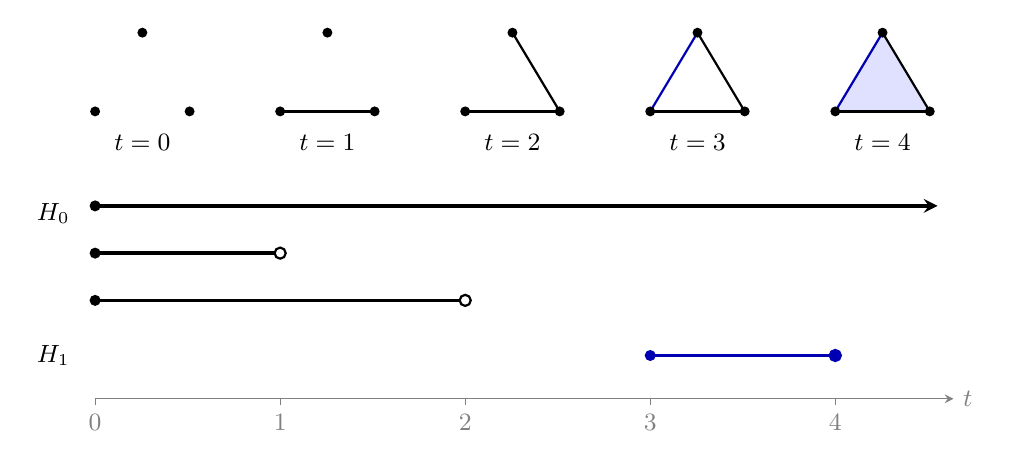
\begin{tikzpicture}[>=stealth,every node/.style={font=\small},x=1cm,y=1cm]
	\foreach \k in {0,1,2,3,4} {
		\begin{scope}[xshift={2.35*\k cm}]
			\ifnum\k=4 \fill[blue!12] (0,0)--(1.2,0)--(.6,1)--cycle;\fi
			\ifnum\k>0 \draw[thick] (0,0)--(1.2,0);\fi
			\ifnum\k>1 \draw[thick] (1.2,0)--(.6,1);\fi
			\ifnum\k>2 \draw[thick,blue!70!black] (.6,1)--(0,0);\fi
			\foreach \p in {(0,0),(1.2,0),(.6,1)} \fill \p circle (1.8pt);
			\node at (.6,-.4) {\(t=\k\)};
		\end{scope}
	}
	\node[left] at (-.2,-1.3) {\(H_0\)};
	\node[left] at (-.2,-3.1) {\(H_1\)};
	\draw[gray,->] (0,-3.65)--(10.9,-3.65) node[right] {\(t\)};
	\foreach \k in {0,1,2,3,4} {
		\draw[gray] ({2.35*\k},-3.65)--({2.35*\k},-3.73) node[below] {\(\k\)};
	}
	\draw[very thick,->] (0,-1.2)--(10.7,-1.2);
	\fill (0,-1.2) circle (2pt);
	\draw[very thick] (0,-1.8)--(2.35,-1.8);
	\fill (0,-1.8) circle (2pt);
	\draw[fill=white,thick] (2.35,-1.8) circle (2pt);
	\draw[very thick] (0,-2.4)--(4.7,-2.4);
	\fill (0,-2.4) circle (2pt);
	\draw[fill=white,thick] (4.7,-2.4) circle (2pt);
	\draw[very thick,blue!70!black] (7.05,-3.1)--(9.4,-3.1);
	\fill[blue!70!black] (7.05,-3.1) circle (2pt);
	\draw[fill=white,thick,blue!70!black] (9.4,-3.1) circle (2pt);
\end{tikzpicture}

	\caption{三角形滤过及其条形码。实心端点表示出生时刻计入区间，空心端点表示死亡时刻已不属于区间。}
	\label{g2:fig:persistence-triangle}
\end{figure}

\subsection{域系数条形码的分解}
\label{g2:subsec:C03:02}

“一个类从出生保持到死亡”可以写成最简单的持续模。给定 \(b<d\leq\infty\)，定义\term[qujianmo]{区间模}[interval module]
\[
	I[b,d)_t=\begin{cases}F,&b\leq t<d,\\0,&\text{其余情形},\end{cases}
\]
两个参数都在区间内时，结构映射为恒等映射，其余结构映射为零。它只携带一个在指定时间段存在的独立方向。下述定理说明，有限构造型持续模正是有限多个这样的方向的直和。

\begin{theorem}[区间分解]\label{g2:thm:finite-persistence-decomposition}
	域 \(F\) 上的每个有限构造型持续模都同构于有限多个区间模 \(I[b,d)\) 的直和，其中 \(b\) 是变化时刻，\(d\) 是较晚的变化时刻或 \(\infty\)。区间及其重数由持续模唯一决定。
\end{theorem}

\begin{proof}
	先证明有限图 \(V_0\to\cdots\to V_N\) 的分解。为便于统一处理最后仍存活的向量，暂时添加 \(V_{N+1}=0\)；这一项只是证明中的记号。用 \(v_i^j\) 表示从第 \(i\) 项到第 \(j\) 项的复合同态。
	\ProseParagraphBreak
	若全部空间为零，结论成立。否则，取最早的非零项 \(V_b\)，选取 \(0\neq x_b\in V_b\)，并令 \(d>b\) 是 \(v_b^d(x_b)=0\) 的最小指标。在 \(b\leq i<d\) 时置 \(x_i=v_b^i(x_b)\)。这些向量非零，并沿箭头依次映到下一项，最后映到零，因而张成一个区间子模。要把它分裂为直和因子，还须选出相容的补空间。
	\ProseParagraphBreak
	选线性泛函 \(\lambda_{d-1}:V_{d-1}\to F\)，使 \(\lambda_{d-1}(x_{d-1})=1\)，并定义
	\[
		\lambda_i=\lambda_{d-1}\circ v_i^{d-1},\qquad b\leq i<d.
	\]
	于是 \(\lambda_i(x_i)=1\)，且 \(\lambda_{i+1}v_i^{i+1}=\lambda_i\)。取 \(W_i=\ker\lambda_i\) 于上述区间内，区间外取 \(W_i=V_i\)。内部箭头保持这些核；入口处 \(V_{b-1}=0\)，出口处目标补空间就是整个 \(V_d\)。故 \(W_i\) 组成子模，且
	\[
		V\cong I[b,d)\oplus W.
	\]
	这里的区间暂以整数指标理解。\(\sum_i\dim W_i<\sum_i\dim V_i\)，反复应用上述步骤便得到有限直和分解。
	\ProseParagraphBreak
	现在证明唯一性。令 \(r(i,j)=\operatorname{rank}v_i^j\)。一个区间 \([b,d)\) 对 \(r(i,j)\) 贡献 \(1\)，当且仅当 \(b\leq i\leq j<d\)。因此，若 \(m_{b,d}\) 为该区间的重数，则
	\[
		r(i,j)=\sum_{b\leq i,\,d>j}m_{b,d}.
	\]
	先取关于 \(i\) 的差，选出恰在 \(b\) 出生的区间；再取关于 \(j\) 的差，选出恰在 \(d\) 死亡的区间。由此得到
	\begin{equation}\label{g2:eq:persistence-multiplicity}
		m_{b,d}=r(b,d-1)-r(b-1,d-1)-r(b,d)+r(b-1,d),
	\end{equation}
	其中 \(r(-1,j)=0\)，添加的零项使 \(r(i,N+1)=0\)。所有重数因而都由原来的映射决定。
	\ProseParagraphBreak
	最后把指标 \(i\) 换回变化时刻 \(a_i\)。死亡指标 \(d\leq N\) 对应实区间 \([a_b,a_d)\)；死亡指标 \(N+1\) 表示在最后一项仍存活，应对应 \([a_b,\infty)\)。在相邻变化时刻之间使用恒等映射延拓，便得到实参数的分解与唯一性。
\end{proof}

\begin{definition}\label{g2:def:persistence-barcode}
	\cref{g2:thm:finite-persistence-decomposition}中带重数的区间集合称为持续模的\term[tiaoxingma]{条形码}[barcode]，记为 \(\mathcal B(V)\)。把每个有限区间 \([b,d)\) 画成平面上的点 \((b,d)\)，并另行保留 \((b,\infty)\)，得到它的\term[chixutu]{持续图}[persistence diagram]。
	\symidx{\(\mathcal B(V)\)：持续模 \(V\) 的条形码}
\end{definition}

分解中选出的向量与补空间可以改变，但区间重数不会改变。特别地，\(\dim V_t\) 等于覆盖时刻 \(t\) 的条数，而 \(\operatorname{rank}v_s^t\) 等于同时覆盖 \(s,t\) 的条数。只给每个时刻的维数会丢失后一项信息，\cref{g2:ex:persistence-same-betti}给出一个只有三个时刻的例子。

\ProseParagraphBreak

也可以把离散持续模写成分次 \(F[u]\)-模 \(\bigoplus_{i\geq0}V_i\)，规定 \(u\cdot x=v_i^{i+1}(x)\) 对 \(x\in V_i\) 成立，并在最后一项以后恒等延拓。一次乘 \(u\) 就是向后移动一步。区间 \([b,d)\) 对应一个在次数 \(b\) 出生、满足 \(u^{d-b}x=0\) 的生成元；无限区间对应没有这种关系的自由生成元。\(F[u]\) 上的分次模结构定理由此给出另一条分解证明，见\cite[第3节]{ZomorodianCarlsson2005Persistence}。上面的直接证明把所需的补空间选择和唯一性公式都留在线性代数之内。

\subsection{边界矩阵约化}
\label{g2:subsec:C03:03}

若在每个阈值重新求一次同调，再比较这些商空间，计算中会反复处理同一批边界。按单形进入的顺序约化边界矩阵，可以同时得到全部出生和死亡。关键是换基必须保持每一步已经出现的链空间：后来的单形可以减去早先的单形，早先的单形却不能掺入尚未出现的单形。

\ProseParagraphBreak

将所有单形排成 \(\sigma_1,\ldots,\sigma_m\)，使滤过值非递减；相同滤过值时，面排在其真上方面之前。例如可先按维数排序，再任意打破剩余的并列。给每个单形定向，把各维边界统一记在一个 \(m\times m\) 矩阵 \(D\) 中：
\[
	\mathrm d\sigma_j=\sum_iD_{ij}\sigma_i.
\]
当 \(D_{ij}\neq0\) 时有 \(i<j\) 及 \(\dim\sigma_i=\dim\sigma_j-1\)。\cref{g2:def:chain-complex}中的 \(\mathrm d^2=0\) 在这个总链空间上成为
\[
	D^2=0.
\]
矩阵的第 \(j\) 列记为 \(D_j\)。对非零列 \(c\)，令 \(\operatorname{low}(c)\) 表示其最大非零行号；零列不定义 \(\operatorname{low}\)。

\begin{definition}\label{g2:def:persistence-column-reduction}
	\term[bianjiejuzhenyuehua]{边界矩阵约化}[boundary matrix reduction]按 \(j=1,\ldots,m\) 执行以下步骤，并同时记录换基矩阵 \(V\)：
	\begin{enumerate}
		\item 初始化 \(R_j=D_j\)、\(V_j=\mathbf e_j\)，其中 \(\mathbf e_j\) 是第 \(j\) 个坐标向量。
		\item 若 \(R_j\neq0\)，且已有 \(k<j\) 满足 \(\operatorname{low}(R_k)=\operatorname{low}(R_j)=i\)，则作
		\[
			c=\frac{(R_j)_i}{(R_k)_i},\qquad R_j\leftarrow R_j-cR_k,\qquad V_j\leftarrow V_j-cV_k,
		\]
		并对更新后的列重复这一步。
		\item 当 \(R_j=0\)，或它的最大非零行号与所有已处理非零列都不同时，保留该列并转向下一列。
	\end{enumerate}
\end{definition}

每次消元都严格降低当前的最大非零行号，因此循环会终止。只有同维单形的边界列才会有相同的非零行号，所以换基保持链的维数。最终有 \(R=DV\)，其中 \(V\) 是对角元全为 \(1\) 的上三角矩阵；每个前缀的链空间都被 \(V\) 保持。\(R\) 的非零列具有互不相同的最大非零行号，因而线性无关。若采用稠密存储，至多 \(m\) 列、每列至多 \(m\) 次消元、每次至多 \(m\) 次域运算，给出 \(O(m^3)\) 的运算上界。

\begin{lemma}\label{g2:lem:persistence-pivot-birth}
	若 \(\operatorname{low}(R_j)=i\)，则 \(R_i=0\)。此外，\(\dim\sigma_j=\dim\sigma_i+1\)，而同一指标 \(i\) 至多与一个 \(j\) 这样配对。
\end{lemma}

\begin{proof}
	因 \(DR_j=D^2V_j=0\)，并且 \(R_j\) 在第 \(i\) 行的系数非零、在更高行的系数为零，故
	\[
		D_i=-\frac{1}{(R_j)_i}\sum_{\ell<i}(R_j)_\ell D_\ell.
	\]
	因此 \(D_i\) 属于前 \(i-1\) 列的张成空间。前缀内的列操作不改变此空间，而已经约化的非零列彼此线性无关，故第 \(i\) 列约化后只能为零。维数关系由边界降低一维得出，配对唯一性则来自非零列的最大非零行号互不相同。
\end{proof}

\begin{theorem}\label{g2:thm:persistence-reduction-barcode}
	对上述约化结果，每一对 \(\operatorname{low}(R_j)=i\) 给出 \(q=\dim\sigma_i\) 维的区间
	\[
		[\,f(\sigma_i),f(\sigma_j)\,),
	\]
	每一个既满足 \(R_i=0\)、又没有作为任何非零列最大非零行号出现的指标 \(i\)，给出 \(\dim\sigma_i\) 维的区间 \([f(\sigma_i),\infty)\)。删去端点相同的空区间后，所得正是各维持续同调的条形码。
\end{theorem}

\begin{proof}
	把矩阵列视为原来单形基下的链。对于一对 \((i,j)\)，令 \(c=(R_j)_i\)，并取
	\[
		z_i=c^{-1}R_j,\qquad w_j=c^{-1}V_j.
	\]
	于是 \(\mathrm d w_j=z_i\)，且 \(\mathrm d z_i=0\)。链 \(z_i\) 的最大指标为 \(i\)，该项系数为 \(1\)；链 \(w_j\) 的最大指标为 \(j\)，该项系数为 \(c^{-1}\neq0\)。对于没有被配对的零列指标 \(i\)，取 \(z_i=V_i\)，则 \(\mathrm d z_i=R_i=0\)，最大指标仍为 \(i\)。
	\ProseParagraphBreak
	由\cref{g2:lem:persistence-pivot-birth}，配对的左端不会又成为某一对的右端，每个指标恰被上述一个向量占据。这些向量相对于原单形基构成上三角且对角元非零的换基，所以在每个前缀内仍是一组基。边界在这组基上只有 \(w_j\mapsto z_i\mapsto0\) 以及未配对的 \(z_i\mapsto0\)。
	\ProseParagraphBreak
	因此，整个滤过链复形分裂为若干基本块。在一个配对块中，\(z_i\) 出现之前没有链；\(z_i\) 出现后有一个 \(q\) 维同调类；\(w_j\) 出现时，该类成为边界，且二者组成的块同调为零。未配对块则在 \(z_i\) 出现以后始终贡献一个同调类。取同调便得到所述区间。
	\ProseParagraphBreak
	若 \(f(\sigma_i)=f(\sigma_j)\)，两条链在同一真实参数同时出现，该块始终没有同调，所以它贡献空区间。相同滤过值内的排序可能改变具体配对；实际实参数持续模保持不变，\cref{g2:thm:finite-persistence-decomposition}保证删去空区间后的条形码保持不变。
\end{proof}

这个证明还给出了区间的循环代表 \(z_i\)。配对只用 \(R\) 即可读取，要恢复这些代表的填充链 \(w_j\)，则保留同步计算的 \(V\)。注意 \(R=DV\) 只改变了列基；证明所用的零关系是 \(DR=0\)。完整的链换基在上一证明中构造。列消元与分次模方法的关系可参见\cite[第4节]{ZomorodianCarlsson2005Persistence}。

\begin{example}\label{g2:exm:persistence-triangle-reduction}
	对\cref{g2:exm:persistence-triangle}，取顺序
	\[
		v_0,v_1,v_2,e_{01},e_{12},e_{02},\tau.
	\]
	其边界矩阵是
	\[
		D=\begin{pmatrix}
			0&0&0&-1&0&-1&0\\
			0&0&0&1&-1&0&0\\
			0&0&0&0&1&1&0\\
			0&0&0&0&0&0&1\\
			0&0&0&0&0&0&1\\
			0&0&0&0&0&0&-1\\
			0&0&0&0&0&0&0
		\end{pmatrix}.
	\]
	前三列为零；第四列最大非零行为 \(2\)，第五列为 \(3\)。第六列先减去第五列，再减去第四列：
	\[
		D_6-D_5-D_4=(v_2-v_0)-(v_2-v_1)-(v_1-v_0)=0.
	\]
	所以 \(R_6=0\)，同步记录的循环是 \(V_6=e_{02}-e_{12}-e_{01}=-z\)。第七列的最大非零行为 \(6\)，此前没有相同的最大非零行，故保持不变。最终配对为
	\[
		(2,4),\qquad(3,5),\qquad(6,7),
	\]
	未配对零列只有第 \(1\) 列。因此零维条形码为 \(\{[0,1),[0,2),[0,\infty)\}\)，一维条形码为 \(\{[3,4)\}\)。相应的死亡链可分别取 \(e_{01},e_{12},-\tau\)，其边界为 \(v_1-v_0,v_2-v_1,-z\)。这直接解释了两次分支合并及一次圈被填满。
\end{example}

\subsection{稳定性需要的距离与有限性条件}
\label{g2:subsec:C03:04}

给滤过值加一点误差，出生和死亡时刻通常也会移动。一个非常短的区间还可能完全消失。因此，比较两张条形码时，既要允许端点移动，也要允许以与长度相称的代价删除短区间。持续图中的对角线正好记录后一种操作。

\begin{definition}\label{g2:def:barcode-bottleneck}
	设 \(\mathcal B,\mathcal C\) 是两张有限条形码，其中每个区间为 \([b,d)\)，允许 \(d=\infty\)。一个\term[bufenpipei]{部分匹配}[partial matching]在两边各选一些区间，并将它们一一配对，重复区间按不同的副本计数。两个有限区间的配对代价为
	\[
		c([b,d),[b',d'))=\max\{|b-b'|,|d-d'|\}.
	\]
	两个无限区间的配对代价为 \(|b-b'|\)，有限区间与无限区间的配对代价为 \(\infty\)。未匹配的有限区间代价为 \((d-b)/2\)，未匹配的无限区间代价为 \(\infty\)。一个部分匹配的代价取上述所有代价的最大值；全空时为零。\term[pingjingjuli]{瓶颈距离}[bottleneck distance]定义为
	\[
		d_{\mathrm B}(\mathcal B,\mathcal C)=\inf_{\text{部分匹配}}\{\text{匹配代价}\}.
	\]
	\symidx{\(d_{\mathrm B}\)：条形码的瓶颈距离}
\end{definition}

对于有限条形码，部分匹配只有有限种，因此上式的下确界能够达到。未匹配区间的代价来自
\[
	\inf_{x\in\mathbb R}\max\{|b-x|,|d-x|\}=\frac{d-b}{2},
\]
最小值在 \(x=(b+d)/2\) 取得。故可以把一个未匹配区间理解为持续图的点 \((b,d)\) 匹配到对角线 \(b=d\)，对角线允许无限重数。无限长区间必须与无限长区间配对，才能有有限距离；最终同调的维数因而也受到控制。

\begin{definition}\label{g2:def:persistence-interleaving}
	给定持续模 \((V,v)\)、\((W,w)\) 和 \(\varepsilon\geq0\)，一个\term[jiaocuo]{交错}[interleaving]由线性映射
	\[
		\alpha_t:V_t\longrightarrow W_{t+\varepsilon},\qquad
		\beta_t:W_t\longrightarrow V_{t+\varepsilon}
	\]
	组成，要求它们与结构映射相容，即对 \(s\leq t\) 有
	\[
		w_{s+\varepsilon}^{t+\varepsilon}\alpha_s=\alpha_t v_s^t,
		\qquad v_{s+\varepsilon}^{t+\varepsilon}\beta_s=\beta_t w_s^t,
	\]
	并且往返一次等于前移 \(2\varepsilon\)：
	\[
		\beta_{t+\varepsilon}\alpha_t=v_t^{t+2\varepsilon},\qquad
		\alpha_{t+\varepsilon}\beta_t=w_t^{t+2\varepsilon}.
	\]
	存在这些映射时称二者 \(\varepsilon\)-交错。\term[jiaocuojuli]{交错距离}[interleaving distance]是所有可行 \(\varepsilon\) 的下确界，记为 \(d_{\mathrm I}(V,W)\)，无可行值时取 \(\infty\)。
	\symidx{\(d_{\mathrm I}\)：持续模的交错距离}
\end{definition}

交错把“两个滤过相差至多一个时间误差”写成了线性映射。往返关系保证来回比较之后，得到的仍是原来同调类向后传递的结果。

\begin{proposition}\label{g2:prop:filtration-sup-interleaving}
	设 \(f,g\) 是同一个有限单纯复形 \(K\) 上的两个滤过函数。若
	\[
		\|f-g\|_\infty=\max_{\sigma\in K}|f(\sigma)-g(\sigma)|\leq\varepsilon,
	\]
	则各维域系数持续同调 \(H_q(K^f_\bullet;F)\) 与 \(H_q(K^g_\bullet;F)\) 是 \(\varepsilon\)-交错的。
\end{proposition}

\begin{proof}
	若 \(f(\sigma)\leq t\)，则 \(g(\sigma)\leq t+\varepsilon\)。交换 \(f,g\) 也成立，所以对每个 \(t\) 都有
	\[
		K^f_t\subseteq K^g_{t+\varepsilon}\subseteq K^f_{t+2\varepsilon},\qquad
		K^g_t\subseteq K^f_{t+\varepsilon}\subseteq K^g_{t+2\varepsilon}.
	\]
	第一步包含诱导 \(\alpha_t,\beta_t\)。所有箭头都是同一复形中子复形的包含，故它们随 \(t\) 相容；两次包含的复合正是原滤过前移 \(2\varepsilon\) 的包含。取同调即得交错的全部等式。
\end{proof}

从条形码匹配也能构造交错。下面先证明这个方向，以看清短区间代价中的因子 \(1/2\) 是怎样出现的。

\begin{proposition}\label{g2:prop:matching-implies-interleaving}
	对有限构造型持续模，有
	\[
		d_{\mathrm I}(V,W)\leq d_{\mathrm B}(\mathcal B(V),\mathcal B(W)).
	\]
\end{proposition}

\begin{proof}
	取一个代价不超过 \(\varepsilon\) 的部分匹配。对于配对区间 \(I[b,d)\)、\(I[b',d')\)，定义 \(\alpha_t\) 在源与平移后的目标都为 \(F\) 时为恒等映射，其余时为零；反向 \(\beta_t\) 同样定义。端点估计给出 \(b'-\varepsilon\leq b\) 和 \(d'-\varepsilon\leq d\)，所以平移后的目标不会比源更晚开始或更晚结束。这正保证重叠处的恒等映射与结构映射相容。
	\ProseParagraphBreak
	如果 \(t,t+2\varepsilon\in[b,d)\)，则端点估计又给出 \(t+\varepsilon\in[b',d')\)，故往返映射为恒等；其余情况源或最终目标为零，往返映射与结构映射都为零。无限区间的检查相同，只需使用出生端点的不等式。
	\ProseParagraphBreak
	对于未匹配的区间，\(d-b\leq2\varepsilon\)，故它从任意 \(t\) 到 \(t+2\varepsilon\) 的结构映射均为零。它与零模通过零映射组成 \(\varepsilon\)-交错。把各个区间的交错取直和，得到 \(V,W\) 的 \(\varepsilon\)-交错。对匹配代价取下确界便得结论。
\end{proof}

反过来，从两组相容线性映射恢复一一匹配，还需要一个匹配定理。单独比较各时刻的维数不足以完成这一步，因为匹配要同时控制所有区间的两端。

\begin{theorem}[持续模等距定理]\label{g2:thm:persistence-isometry}
	对于同一域上两个有限构造型持续模 \(V,W\)，有
	\[
		d_{\mathrm B}(\mathcal B(V),\mathcal B(W))=d_{\mathrm I}(V,W).
	\]
\end{theorem}

这里引用\cite[第5章，The Isometry Theorem]{ChazalDeSilvaGlisseOudot2016}的等距定理。其代数稳定性方向把交错产生的秩约束转化为区间匹配；与\cref{g2:prop:matching-implies-interleaving}合起来得到上式。书中的定理覆盖更一般的持续模，本节的有限维、有限变化时刻以及左闭右开约定保证可直接应用。特别地，如果存在一个 \(\varepsilon\)-交错，则瓶颈距离至多为 \(\varepsilon\)；有限条形码的最优部分匹配存在，所以能实际选出代价至多为 \(\varepsilon\) 的匹配。

\begin{corollary}\label{g2:cor:finite-filtration-stability}
	同一个有限单纯复形上的滤过函数 \(f,g\) 满足
	\[
		d_{\mathrm B}\bigl(\mathcal B(H_q(K^f_\bullet;F)),\mathcal B(H_q(K^g_\bullet;F))\bigr)
		\leq\|f-g\|_\infty.
	\]
\end{corollary}

\begin{proof}
	\cref{g2:prop:filtration-sup-interleaving}给出以 \(\|f-g\|_\infty\) 为参数的交错，\cref{g2:thm:persistence-isometry}把它转化为同样界限的瓶颈距离。
\end{proof}

例如，三角形中若所有滤过值的误差至多为 \(\varepsilon<1/2\)，原来的一维区间 \([3,4)\) 长度大于 \(2\varepsilon\)，便不能以允许的代价匹配到对角线，必须有另一个一维区间与它配对，且出生和死亡时刻分别相差至多 \(\varepsilon\)。长度不超过 \(2\varepsilon\) 的区间则可能消失。这一结论把测量误差与可追踪的同调特征长度联系起来。

\ProseParagraphBreak

本节的假设各有具体作用。域系数保证线性泛函、补空间及除法消元都可使用；有限单形数保证算法终止，且条形码只有有限条；实参数上在变化时刻采用变化后的值，使区间统一为左闭右开；距离中允许匹配到对角线，则容纳了短寿命特征的消失。把整数系数直接代入区间分解会遗漏映射中的整除信息，\cref{g2:ex:persistence-integer-obstruction}将这一点化为一个乘 \(2\) 的例子。

\begin{chaptersummary}
	\begin{itemize}
		\item Borel 构造 \(X_G=EG\times_GX\) 是 \(BG\) 上纤维为 \(X\) 的丛。自由主作用给出普通商的上同调，固定点保留 \(H^*(BG)\)。圆群等变球面满足 \(x(x+u)=0\)，固定点限制的像由整除关系控制。
		\item Cartan 模型将多项式元置于偶数次数，以外微分和内乘组成等变微分。紧性、不变性及系数约定保证它与 Borel 模型的比较；环面局部化通过倒置非零权消去非固定轨道的贡献。
		\item 谱的结构映射组织悬挂过渡，稳定同伦群由相应直极限给出。球谱、普通同调谱和 K 理论谱具有不同的系数；广义同调的正合性与表示需要所选稳定范畴的基础定理。
		\item 有限滤过的同调及诱导映射组成持续模。域系数下的区间分解保存各同调类的生存范围，区间重数由秩数据决定；只有每一步的 Betti 数不足以恢复这些信息。
		\item 边界矩阵约化通过保持过滤次序的列变换读出生死配对。过滤值的统一扰动界先给交错，再由匹配定理得到瓶颈距离估计，半开区间、零长区间和无限条均按同一约定处理。
	\end{itemize}
\end{chaptersummary}

\BookExercises

\begin{exercise}\label{g2:ex:equivariant-hopf-sphere}
	圆群 \(T\) 在 \(S^{2m+1}\subset\mathbb C^{m+1}\) 上按标量左乘，\(m\ge0\)。用自由作用商和球丛 Gysin 序列两种方法计算 \(H_T^*(S^{2m+1};\mathbb Z)\)。在商 \(\mathbb CP^m\) 上取 \(h=c_1(\gamma^*)\)，核对来自 \(BT\) 的 \(u\) 对应于 \(h\) 还是 \(-h\)。
\end{exercise}
\begin{solution}
	作用自由，Hopf 轨道映射是主丛，所以\cref{g2:prop:free-action-borel-quotient}给出 \(H_T^*(S^{2m+1};\mathbb Z)=H^*(\mathbb CP^m;\mathbb Z)=\mathbb Z[h]/(h^{m+1})\)。要比较 \(u\)，将左主丛改写为右主丛 \(Q\)，令 \(x\cdot z=z^{-1}x\)。其权 \(1\) 关联线是 \(\gamma^*\)：若 \(\ell_x\) 是 \(\mathbb Cx\) 上满足 \(\ell_x(x)=1\) 的复线性泛函，则
	\[
		[x,w]\longmapsto w\ell_x
	\]
	良定义，因为 \(\ell_{z^{-1}x}=z\ell_x\)。在 Borel 构造到 \(BT\) 和到 \(\mathbb CP^m\) 的两张投影下，所拉回的主右丛同构，故 \(u\) 对应 \(c_1(\gamma^*)=h\)。这里右作用的转换解释了为何与 \(BT\) 上 \(u=c_1(\gamma)\) 的写法不矛盾。

	另一方面，Borel 构造是 \(BT\) 上复秩 \(m+1\) 丛 \(L^{\oplus(m+1)}\) 的单位球丛。其底层定向实丛的 Euler 类为顶陈类 \(u^{m+1}\)。\cref{g2:thm:thom-gysin}中乘 \(u^{m+1}\) 的映射在 \(\mathbb Z[u]\) 上单射，因此总空间的上同调由其余核给出，且由底空间拉回生成。所得环为
	\[
		H_T^*(S^{2m+1};\mathbb Z)=\mathbb Z[u]/(u^{m+1}),
	\]
	与第一种方法及 \(u\leftrightarrow h\) 的对应一致。
\end{solution}

\begin{exercise}\label{g2:ex:weighted-sphere-coefficients}
	设 \(m\ge2\)，圆群按 \(z\cdot[z_0:z_1]=[z_0:z^m z_1]\) 作用于 \(\mathbb CP^1\)。计算整系数等变上同调环及固定点限制的像。若素数 \(p\mid m\)，改用 \(\mathbb F_p\) 系数后，证明固定点限制即使倒置 \(u\) 仍不是单射。比较有理系数下的情形。
\end{exercise}
\begin{solution}
	权 \(m\) 的关联线是 \(L^{\otimes m}\)，第一陈类为 \(mu\)。Borel 构造因而是 \(\mathbb P(\underline{\mathbb C}\oplus L^{\otimes m})\)。取重言对偶的一阶类 \(x\)，射影丛公式给出
	\[
		H_T^*(\mathbb CP^1;\mathbb Z)=\mathbb Z[u,x]/\bigl(x(x+mu)\bigr),
	\]
	并以 \(1,x\) 为 \(\mathbb Z[u]\) 模基。两个固定点限制为 \(x|_N=0\)、\(x|_S=-mu\)，所以像为 \(P-Q\in mu\mathbb Z[u]\) 的多项式对。由于 \(mu\) 非零且不是零因子，整系数限制仍单射，但只倒置 \(u\) 后其像仍要求差属于 \(m\mathbb Z[u,u^{-1}]\)。

	改用 \(\mathbb F_p\) 后，整数上同调无挠，万有系数定理或射影丛基直接给出 \(\mathbb F_p[u,x]/(x^2)\)。其中非零的 \(x\) 限制为 \((0,0)\)，它又是自由模基的一项，故倒置 \(u\) 后仍非零。若采用有理系数，\(m\) 已可逆，继续倒置 \(u\) 便可解任意 \(P-Q=mu b\)，因此限制变为同构。有限稳定子中的 \(m\) 扭信息决定了这三种系数下的差别。
\end{solution}

\begin{exercise}\label{g2:ex:finite-isotropy-orbit}
	设 \(C_m\subset T=S^1\) 是 \(m\) 次单位根群，\(m\ge2\)。计算轨道 \(T/C_m\) 的整系数与有理系数等变上同调，并说明为什么其轨道空间的一点不能恢复整系数答案。
\end{exercise}
\begin{solution}
	由\cref{g2:prop:borel-homogeneous-orbit}，所求为 \(H^*(BC_m)\)。将 \(T/C_m\) 识别为单位圆时，可用 \(zC_m\mapsto z^m\)，所以 \(T\) 作用成为权 \(m\) 的旋转。其 Borel 构造是 \(L^{\otimes m}\) 的单位圆丛，Euler 类为 \(mu\)。Gysin 序列中的乘法 \(\mathbb Z[u]\xrightarrow{mu}\mathbb Z[u]\) 单射，故奇次群为零，零次为 \(\mathbb Z\)，每个正偶次为 \(\mathbb Z/m\)。这些类均由底空间拉回的 \(u\) 的幂生成，得到
	\[
		H_T^*(T/C_m;\mathbb Z)\cong\mathbb Z[u]/(mu).
	\]
	有理化后 \(m\) 可逆，关系强迫 \(u=0\)，所以只剩零次的 \(\mathbb Q\)。普通轨道空间是一点，其整数上同调没有这些正次扭类；扭类记录的是被普通取商压去的有限稳定子。
\end{solution}

\begin{exercise}\label{g2:ex:cartan-free-torus}
	令 \(T=S^1\) 作用于 \(M=(\mathbb R/\mathbb Z)^2\)，作用为 \(t\cdot(\theta,\varphi)=(\theta+t,\varphi)\)。直接计算 Cartan 复形的上同调环，并与商空间的 de Rham 上同调比较。指出复形中 \(\mathrm d\theta\) 与 \(\mathrm d\varphi\) 的不同作用。
\end{exercise}
\begin{solution}
	沿 \(\theta\) 平移不变的形式，其系数只依赖 \(\varphi\)。因此整个复形是分次张量积
	\[
		\bigl(\mathbb R[u]\otimes\Lambda(\mathrm d\theta),\ \mathrm d_T(\mathrm d\theta)=-u\bigr)
		\otimes\bigl(\Omega(S^1_\varphi),\mathrm d\bigr).
	\]
	第一个因子到 \(\mathbb R\) 的映射把 \(u\) 与 \(\mathrm d\theta\) 都送到零。它是链同伦等价：在多项式基上令 \(h(1)=0\)、\(h(u^j)=-u^{j-1}\mathrm d\theta\)（\(j\ge1\)），并令 \(h(u^j\mathrm d\theta)=0\)，则 \(\mathrm d_T h+h\mathrm d_T\) 等于恒等映射减去常数投影。张量上第二个复形后仍给出链同伦，故上同调环等于
	\[
		H^*(S^1_\varphi;\mathbb R)=\Lambda_{\mathbb R}([\mathrm d\varphi]).
	\]
	这正是自由作用商 \(M/T=S^1_\varphi\) 的上同调。形式 \(\mathrm d\varphi\) 水平且闭，下降为商上的生成元；\(\mathrm d\theta\) 沿轨道不水平，它在等变微分下产生 \(-u\)，使群方向的正次多项式成为边界。
\end{solution}

\begin{exercise}\label{g2:ex:cartan-sphere-lifts}
	采用\cref{g2:ex:cartan-rotating-sphere}的 \(s,\omega,V,u,x\)。求所有满足 \(\mathrm d\mu=\iota_V\omega\) 的光滑函数 \(\mu\)，并在 \(H_T^2(\mathbb CP^1;\mathbb R)\) 中识别 \([\omega+u\mu]\)。其中哪些类来自整数等变上同调？说明在北极规定 \(\mu(N)=0\) 起了什么作用。
\end{exercise}
\begin{solution}
	因为 \(\iota_V\omega=-\mathrm ds\)，方程等价于 \(\mathrm d(\mu+s)=0\)。球面连通，所以全部解为 \(\mu=-s+c\)，其中 \(c\in\mathbb R\)。于是
	\[
		[\omega+u\mu]=[\omega-su]+cu=x+cu.
	\]
	其两极限制分别为 \(cu\) 与 \((c-1)u\)。由\cref{g2:thm:equivariant-sphere-ring}，整数二次群以 \(u,x\) 为自由基，实系数群由它扩张系数得到。因此 \(x+cu\) 是整数类的像，当且仅当 \(c\in\mathbb Z\)。这也能直接从北极限制看出必要性，再用整数基看出充分性。

	条件 \(\mu(N)=0\) 选定 \(c=0\)，从所有普通类为 \([\omega]\) 的等变提升中选出 \(x\)。普通面积形式只能确定微分 \(\mathrm d\mu\)，不能确定加法常数；固定一个点上的值才完成这项归一化。若 \(c\) 为整数，给重言对偶线的等变结构再张量权 \(c\) 的平凡线，其一阶类就是 \(x+cu\)。
\end{solution}

\begin{exercise}\label{g2:ex:localization-noncompact-orbits}
	令 \(T=(S^1)^2\)，并令 \(H_n=\ker\chi_n\)，其中 \(\chi_n(z_1,z_2)=z_1z_2^n\)，\(n=1,2,\ldots\)。在光滑非紧流形 \(M=\coprod_{n\ge1}T/H_n\) 上取逐分支的左作用。证明 \(M^T=\varnothing\)，但对 \(\mathbf k=\mathbb Q\) 或 \(\mathbb R\)，\(S^{-1}H_T^*(M;\mathbf k)\ne0\)，其中 \(S\) 仍由所有非零特征标类生成。解释有限胞腔证明中的哪一步不能用于这个例子。
\end{exercise}
\begin{solution}
	每个 \(H_n\) 都是真一维子环面，故每个轨道均无固定点。空间 \(M\) 是可数个圆的不交并，具有第二可数的一维光滑结构；它不紧。由齐性轨道的 Borel 计算与不交并的上同调，逐次数有
	\[
		H_T^*(M;\mathbf k)=\prod_{n\ge1}H^*(BH_n;\mathbf k).
	\]
	这里乘积按每一个上同调次数理解。以 \(t\mapsto(t^{-n},t)\) 参数化 \(H_n\)，并以 \(v\) 表示 \(H^2(BH_n;\mathbf k)\) 的生成元，则限制为 \(u_1\mapsto-nv\)、\(u_2\mapsto v\)。所以该分支的系数环是
	\[
		\mathbf k[u_1,u_2]/(u_1+nu_2).
	\]
	取零次类 \(\mathbf 1=(1,1,\ldots)\)。任意 \(s\in S\) 是有限个非零整系数线性式的乘积。在第 \(n\) 个分支上，一个因子 \(au_1+bu_2\) 限制为 \((b-an)v\)。若 \(a\ne0\)，它至多在一个正整数 \(n\) 上为零；若 \(a=0\)，则因 \(b\ne0\) 而在所有分支上都非零。故有限个因子的乘积在除有限多个以外的分支上均非零，\(s\mathbf 1\ne0\)。

	因此没有 \(s\in S\) 消灭 \(\mathbf 1\)，局部化中的 \(\mathbf 1/1\) 非零。每个轨道的等变上同调单独都被一个权消灭，但无穷多个轨道需要无穷多个不同的权；乘法集中的分母只有有限个因子。有限胞腔证明所用的有限归纳在这里不能替代为对所有分支的一次统一消灭。
\end{solution}

\begin{exercise}\label{g2:ex:spectrum-degree-two-system}
	令预谱 \(E\) 的第 \(n\) 层为 \(S^n\)，每个结构映射 \(\Sigma S^n=S^{n+1}\to S^{n+1}\) 的度数为 \(2\)。计算 \(\pi_0(E)\) 和所有负次稳定群，并判断它是否与球预谱稳定等价。
\end{exercise}
\begin{solution}
	当 \(n\ge2\) 时，\(\pi_n(S^n)\cong\mathbb Z\) 由度数识别。悬挂保持度数，随后与度数 \(2\) 的结构映射复合使度数乘 \(2\)，所以
	\[
		\pi_0(E)=\varinjlim\bigl(\mathbb Z\xrightarrow{\times2}\mathbb Z\xrightarrow{\times2}\cdots\bigr).
	\]
	把第 \(n\) 项的整数 \(a\) 送到 \(a/2^n\in\mathbb Q\)。这个赋值与过渡相容，因为 \(2a/2^{n+1}=a/2^n\)。所得像为所有分母是二次幂的有理数，即 \(\mathbb Z[1/2]\)。若两个分数相等，乘以足够大的共同二次幂后，两个整数代表就在同一个阶段相等，所以该映射也单射。因此 \(\pi_0(E)\cong\mathbb Z[1/2]\)。

	对 \(q<0\)，充分大的 \(n\) 满足 \(2\le q+n<n\)，球面连通性使各项 \(\pi_{q+n}(S^n)=0\)，故 \(\pi_q(E)=0\)。球预谱的零次稳定群是 \(\mathbb Z\)，与 \(\mathbb Z[1/2]\) 不同构：前者的非零元不可能无限次被 \(2\) 整除，后者的每个元素都可被 \(2\) 整除。因此两者不稳定等价，尽管每层的空间完全相同。
\end{solution}

\begin{exercise}\label{g2:ex:generalized-moore-homology}
	设 \(m\ge2\)、\(r\ge2\)，令 \(M=S^r\cup_m e^{r+1}\)，其中附着映射的度数为 \(m\)。对任意谱 \(E\)，从映射锥长正合列证明有自然短正合列
	\[
		0\longrightarrow\pi_{q-r}(E)/m\pi_{q-r}(E)
		\longrightarrow\widetilde E_q(M)
		\longrightarrow\{a\in\pi_{q-r-1}(E):ma=0\}\longrightarrow0.
	\]
	据此分别计算 \(E=H\mathbb Z\) 与 \(E=KU\) 时的全部群。
\end{exercise}
\begin{solution}
	空间余纤维序列为 \(S^r\xrightarrow{m}S^r\to M\to S^{r+1}\)。稳定范畴中的度 \(m\) 球面映射，是恒等映射在阿贝尔映射群中的 \(m\) 倍，所以在任意广义同调上都作用为乘 \(m\)。用球面系数公式，长正合列的相关部分为
	\[
		\pi_{q-r}(E)\xrightarrow{\times m}\pi_{q-r}(E)
		\longrightarrow\widetilde E_q(M)\longrightarrow
		\pi_{q-r-1}(E)\xrightarrow{\times m}\pi_{q-r-1}(E).
	\]
	在两端取余核和核，即得短正合列。一般情形不能仅凭这条列指定自然分裂。

	对 \(H\mathbb Z\)，系数只在零次为 \(\mathbb Z\)，乘 \(m\) 在 \(\mathbb Z\) 上单射，故 \(\widetilde H_q(M;\mathbb Z)\) 只在 \(q=r\) 为 \(\mathbb Z/m\)，其余为零。对 \(KU\)，所有系数均无 \(m\) 挠元，右端核为零；偶次系数为 \(\mathbb Z\)，奇次为零，因此
	\[
		\widetilde{KU}_q(M)=
		\begin{cases}\mathbb Z/m,&q-r\text{ 为偶数},\\0,&q-r\text{ 为奇数}.
		\end{cases}
	\]
	这个结果对所有整数 \(q\) 成立。同一张附着映射在普通理论中只留下一个次数的挠群，在复 \(K\) 同调中则按二周期重复出现。
\end{solution}

\begin{exercise}\label{g2:ex:stable-wedge-direct-sum-product}
	令 \(X=\bigvee_{j=1}^{\infty}S^2\)，带 CW 弱拓扑。计算 \(\widetilde{KU}_0(X)\) 与 \(\widetilde{KU}^{\,0}(X)\)，并说明为何前者是直和、后者是乘积。比较这两个群的基数。
\end{exercise}
\begin{solution}
	每份二球面的两种群分别为 \(\pi_{-2}(KU)=\mathbb Z\) 与 \(\pi_2(KU)=\mathbb Z\)。\cref{g2:prop:spectrum-exact-wedge}于是给出
	\[
		\widetilde{KU}_0(X)=\bigoplus_{j=1}^{\infty}\mathbb Z,
		\qquad\widetilde{KU}^{\,0}(X)=\prod_{j=1}^{\infty}\mathbb Z.
	\]
	同调的直和意味着每个类只含有限多个分支的非零贡献；这来自球谱的紧性。上同调是从整个楔和到表示谱的映射，余积性质允许在每个分支上独立指定一个整数，没有有限支撑要求，因而得到乘积。

	直和是可数集：按有限支撑所在的最大下标取可数并，每个部分包含于某个有限次 \(\mathbb Z^N\)。乘积包含全部二进制序列 \(\{0,1\}^{\mathbb N}\)，由对角线论证是不可数集。因此两个群甚至不可能作为集合双射，更不可能同构。有限楔和时直和与乘积相同，不能由有限例子省略无限楔和公理的区别。
\end{solution}

\begin{exercise}\label{g2:ex:persistence-same-betti}
	考虑两个在时刻 \(0,1,2\) 分别为 \(F,F^2,F\) 的持续模，最早时刻之前为零，最后时刻以后恒等延拓。第一个箭头均为 \(x\mapsto(x,0)\)，第二个箭头分别为 \((a,b)\mapsto a\) 和 \((a,b)\mapsto b\)。计算两张条形码及从时刻 \(0\) 到时刻 \(2\) 的秩，并说明各时刻的 Betti 数为什么不能确定条形码。
\end{exercise}
\begin{solution}
	记 \(F^2\) 的标准基为 \(e_1,e_2\)。第一种情形中，时刻 \(0\) 的生成元依次映为 \(e_1\) 和 \(1\)，始终存活；\(e_2\) 在时刻 \(1\) 出生，下一步映为零。所以条形码是
	\[
		\{[0,\infty),[1,2)\},\qquad r(0,2)=1.
	\]
	第二种情形中，时刻 \(0\) 的生成元映为 \(e_1\)，随后死亡；时刻 \(1\) 新出现的 \(e_2\) 映为末项的 \(1\)，以后始终存活。因此条形码是
	\[
		\{[0,2),[1,\infty)\},\qquad r(0,2)=0.
	\]
	两者各时刻的维数都是 \(1,2,1\)，但第一个持续模把最早的类保留到最后，第二个则以一个新类接替它。条形码记录的映射信息正体现在这个差别上。
\end{solution}

\begin{exercise}\label{g2:ex:persistence-square}
	用对角线 \(ac\) 将四边形 \(abcd\) 分为三角形 \(abc,acd\)。令所有顶点在 \(0\) 出现，四条外边在 \(1\) 出现，对角线在 \(2\) 出现，两个面分别在 \(3,4\) 出现。计算各维条形码，并给出两个一维区间的循环代表及死亡链。若把对角线与面 \(abc\) 的滤过值都改为 \(3\)，条形码怎样变化？
\end{exercise}
\begin{solution}
	把外边定向为 \(e_{ab},e_{bc},e_{cd},e_{ad}\)，对角线定向为 \(e_{ac}\)。时刻 \(1\) 的外圈是
	\[
		z=e_{ab}+e_{bc}+e_{cd}-e_{ad}.
	\]
	这是连通图中唯一的独立圈：图有 \(4\) 条边、\(4\) 个顶点，边界矩阵秩为 \(3\)，故一维循环空间维数为 \(1\)。对角线出现后，新增独立循环
	\[
		y=e_{ab}+e_{bc}-e_{ac}.
	\]
	它与 \(z\) 独立，因为 \(y\) 的对角线系数非零，而 \(z\) 的该系数为零。两个面的边界为
	\[
		\mathrm d[abc]=y,\qquad \mathrm d[acd]=z-y.
	\]
	在时刻 \(3\)，\(y\) 被填掉，\(z\) 仍非零；在时刻 \(4\)，\(z=\mathrm d([abc]+[acd])\) 也被填掉。因此
	\[
		\mathcal B(H_1)=\{[1,4),[2,3)\}.
	\]
	循环代表可取 \(z,y\)，死亡链分别为 \([abc]+[acd]\) 和 \([abc]\)。时刻 \(1\) 四个顶点同时连成一个分支，所以
	\[
		\mathcal B(H_0)=\{[0,\infty),[0,1),[0,1),[0,1)\}.
	\]
	两个二维面的边界独立，故 \(H_2=0\)，更高维也为零。
	\ProseParagraphBreak
	若对角线与第一个面同时在 \(3\) 出现，新增的链 \(y\) 立即成为该面的边界，不在任何参数处贡献同调。矩阵排序会给出空区间 \([3,3)\)，删除后只剩 \(\mathcal B(H_1)=\{[1,4)\}\)；零维条形码不变。
\end{solution}

\begin{exercise}\label{g2:ex:persistence-distance-zero}
	设 \(V\) 是具有有限条形码的持续模。直接从定义证明，\(V\) 到零模的交错距离等于条形码中最长有限区间长度的一半；若存在无限区间，则距离为 \(\infty\)。全空条形码的距离约定为零。再计算 \(\{[0,L)\}\) 与 \(\{[h,L+h)\}\) 的瓶颈距离，其中 \(L>0\)、\(h\geq0\)。
\end{exercise}
\begin{solution}
	与零模之间的两组映射只能是零映射。因此存在 \(\varepsilon\)-交错，当且仅当所有结构映射 \(v_t^{t+2\varepsilon}\) 都为零。区间 \([b,d)\) 满足此条件，当且仅当 \(d-b\leq2\varepsilon\)：若严格长于 \(2\varepsilon\)，取 \(t=b\)，结构映射为恒等；若长度不超过 \(2\varepsilon\)，\(t\) 和 \(t+2\varepsilon\) 不可能同时落在该左闭右开区间内。取有限直和，便得到所述最长长度公式。无限区间在任意有限前移后仍有非零结构映射，所以不存在有限交错参数。
	\ProseParagraphBreak
	对于题中的两张单区间条形码，部分匹配只有两种实质选择：将两条配对，代价为 \(h\)；或两条都匹配到对角线，代价为 \(L/2\)。因此
	\[
		d_{\mathrm B}\bigl(\{[0,L)\},\{[h,L+h)\}\bigr)=\min\{h,L/2\}.
	\]
	当位移很大时，最优匹配会把两条都送到对角线。这说明瓶颈距离同时衡量端点移动与特征消失的代价。
\end{solution}

\begin{exercise}\label{g2:ex:persistence-integer-obstruction}
	把两项持续模 \(\mathbb Z\xrightarrow{\times2}\mathbb Z\) 与 \(\mathbb Z\xrightarrow{\mathrm{id}}\mathbb Z\) 比较，证明它们不同构，虽然各项及箭头的秩相同。再证明前者不能分解为整数区间模的直和，其中整数区间模在区间内取 \(\mathbb Z\)，内部映射取恒等。最后将系数分别换为 \(\mathbb Q\) 和 \(\mathbb F_2\)，计算前者的条形码；两时刻取 \(0,1\)，此前为零、此后恒等延拓。
\end{exercise}
\begin{solution}
	两个箭头的余核分别为 \(\mathbb Z/2\mathbb Z\) 和零，持续模同构会诱导箭头余核的同构，所以它们不同构。它们的两个对象秩都为 \(1\)，箭头的像也都秩为 \(1\)；秩没有记录像 \(2\mathbb Z\) 在目标中的指数。
	\ProseParagraphBreak
	若第一个图能分解为整数区间模，第一项秩为 \(1\) 表明恰有一条区间覆盖时刻 \(0\)。箭头非零要求这条区间也覆盖时刻 \(1\)；末项秩为 \(1\) 又排除了其他区间。于是箭头在某组整数基下应为恒等，其余核为零，与 \(\mathbb Z/2\mathbb Z\) 矛盾。
	\ProseParagraphBreak
	换为 \(\mathbb Q\) 后，乘 \(2\) 是同构，选择末项的基向量为 \(2\) 即把箭头写成恒等，条形码为 \(\{[0,\infty)\}\)。换为 \(\mathbb F_2\) 后，箭头为零，第一个类在 \(1\) 死亡，末项出现另一个类，条形码为 \(\{[0,1),[1,\infty)\}\)。域系数既使区间分解成立，也会影响实际得到的条形码。
\end{solution}
